\documentclass[12pt,a4paper]{article}

% ── Page layout ───────────────────────────────────────────────────────────────
\usepackage[top=1in, bottom=1in, left=1.25in, right=1in]{geometry}

% ── Typography ────────────────────────────────────────────────────────────────
\usepackage{lmodern}
\usepackage[T1]{fontenc}
\usepackage[utf8]{inputenc}
\usepackage{textcomp}
\usepackage{microtype}
\usepackage{setspace}
\onehalfspacing

% ── Headers / footers ─────────────────────────────────────────────────────────
\usepackage{fancyhdr}
\setlength{\headheight}{14pt}
\pagestyle{fancy}
\fancyhf{}
\lhead{\small Optimizer and Learning Rate Simulation}
\rhead{\small HI 192}
\cfoot{\thepage}
\renewcommand{\headrulewidth}{0.4pt}

% ── Section title formatting ──────────────────────────────────────────────────
\usepackage{titlesec}

% ── Math ──────────────────────────────────────────────────────────────────────
\usepackage{amsmath}

% ── Figures ───────────────────────────────────────────────────────────────────
\usepackage{graphicx}
\usepackage{subcaption}
\usepackage{float}
\usepackage{placeins}
\usepackage{pdflscape}
\usepackage{afterpage}
\usepackage{caption}
\captionsetup{font=small, labelfont=bf, justification=raggedright, singlelinecheck=false}
\captionsetup[subfigure]{font=small, justification=centering}

% ── Tables ────────────────────────────────────────────────────────────────────
\usepackage{longtable}
\usepackage{booktabs}
\usepackage{tabularx}
\usepackage{multirow}

% ── Colors ────────────────────────────────────────────────────────────────────
\usepackage[dvipsnames,svgnames,x11names,table,HTML]{xcolor}
\colorlet{tableheader}{gray!15}
\definecolor{linkblue}{RGB}{0,70,140}

% ── Code listings ─────────────────────────────────────────────────────────────
\usepackage{listings}
\lstdefinestyle{python}{
  language=Python,
  basicstyle=\scriptsize\ttfamily,
  keywordstyle=\bfseries,
  commentstyle=\itshape,
  numbers=left,
  numberstyle=\tiny,
  numbersep=5pt,
  frame=tb,
  xleftmargin=2em,
  framexleftmargin=1.5em,
  breaklines=true,
  showstringspaces=false,
  literate=
    {─}{{-}}1
    {━}{{-}}1
    {│}{{|}}1
    {✓}{{[ok]}}1
    {✗}{{[x]}}1
    {→}{{->}}1
    {…}{{...}}1
    {×}{{x}}1
    {≥}{{>=}}1
    {≤}{{<=}}1
    {≠}{{!=}}1,
}

% ── TikZ ──────────────────────────────────────────────────────────────────────
\usepackage{tikz}
\usetikzlibrary{shapes.geometric, arrows.meta, positioning, fit, backgrounds}

% ── Appendices ────────────────────────────────────────────────────────────────
\usepackage{appendix}

% ── Hyperlinks (load last) ────────────────────────────────────────────────────
\usepackage[
  colorlinks=true,
  linkcolor=linkblue,
  citecolor=linkblue,
  urlcolor=linkblue,
  pdftitle={Optimizer and Learning Rate Study of Ovarian Cancer Prediction},
  pdfauthor={DelaCruz, Doria, Rodriguez},
]{hyperref}

% ── Custom commands ───────────────────────────────────────────────────────────
\newcommand{\codefile}[1]{\vspace{0.5em}\noindent\textbf{\small\texttt{#1}}\vspace{0.2em}\par}
\newcommand{\metricrow}[7]{#1 & #2 & #3 & #4 & #5 & #6 & #7}

% ─────────────────────────────────────────────────────────────────────────────
\begin{document}

% ── Title page ────────────────────────────────────────────────────────────────
\begin{titlepage}
  \centering
  \vspace*{4cm}
  {\LARGE\textbf{Optimizer and Learning Rate Simulation\\[0.4em]of Ovarian Cancer Prediction}\\[1.5em]}
  {\large HI 192: Knowledge Representation and Health Decision Support\\[1.5em]}
  {\large \textbf{DELA CRUZ} James Angelo \quad \textbf{DORIA}, Marc \quad \textbf{RODRIGUEZ}, Augustus Clark Raphael\\[1em]}
  {\large May 2026}
  \vfill
\end{titlepage}

\thispagestyle{empty}
\tableofcontents
\newpage
\listoffigures
\newpage
\listoftables
\newpage

% ── Body sections ─────────────────────────────────────────────────────────────
\newpage
\section{Dataset}
\label{sec:dataset}

\subsection{Sourcing}

The dataset used in this study is the \textbf{STRAMPN Histopathological Images for Ovarian Cancer Prediction}, published on IEEE DataPort and accessible at:

\begin{center}
\url{https://ieee-dataport.org/documents/strampn-histopathological-images-ovarian-cancer-prediction}
\end{center}

The dataset consists of histopathological JPEG images drawn from ovarian tissue specimens and is labelled for binary classification: \emph{Ovarian Cancer} versus \emph{Ovarian Non-Cancer}. The dataset was accessed in May 2026. In accordance with IEEE DataPort terms, the dataset is not redistributed as part of this repository; all rights remain with the original authors.

\subsection{Composition}

The full dataset contains 987 images distributed across two classes as shown in Table~\ref{tab:class-composition}.

\begin{table}[H]
  \centering
  \caption{Class composition of the STRAMPN dataset.}
  \label{tab:class-composition}
  \begin{tabular}{lrr}
    \toprule
    \rowcolor{tableheader}
    \textbf{Class} & \textbf{Count} & \textbf{Percentage} \\
    \midrule
    Ovarian Cancer     & 481 & 48.73\% \\
    Ovarian Non-Cancer & 506 & 51.27\% \\
    \midrule
    \textbf{Total}     & \textbf{987} & \textbf{100\%} \\
    \bottomrule
  \end{tabular}
\end{table}

The class distribution is near-balanced, with a modest majority of non-cancer images (51.27\%). This near-parity reduces the risk of class-imbalance bias and justifies the use of accuracy as a supplementary metric alongside AUC-ROC.

\subsection{Train / Validation / Test Split}

A two-stage stratified split was applied to partition the dataset. In the first stage, 75\% of images per class were assigned to a combined train-and-validation pool, with the remaining 25\% reserved as the held-out test set. In the second stage, the train-and-validation pool was further divided 70\%/30\%, yielding approximately 52.5\% of the full dataset for training and 22.5\% for validation.

Both split stages used \texttt{sklearn.model\_selection.train\_test\_split} with \texttt{stratify=labels} and \texttt{random\_state=42}, ensuring class proportions are preserved in every subset and the split is fully reproducible. The resulting partition is shown in Table~\ref{tab:split}.

\begin{table}[H]
  \centering
  \caption{Stratified train / validation / test split.}
  \label{tab:split}
  \begin{tabular}{lrrrr}
    \toprule
    \rowcolor{tableheader}
    \textbf{Split} & \textbf{Cancer} & \textbf{Non-Cancer} & \textbf{Total} & \textbf{\% of Dataset} \\
    \midrule
    Train      & 253 & 265 & 518 & 52.48\% \\
    Validation & 108 & 114 & 222 & 22.49\% \\
    Test       & 120 & 127 & 247 & 25.03\% \\
    \midrule
    \textbf{Total} & \textbf{481} & \textbf{506} & \textbf{987} & \textbf{100\%} \\
    \bottomrule
  \end{tabular}
\end{table}

The fixed \texttt{random\_state=42} is applied consistently throughout \texttt{src/preprocessing.py} and is never altered between the 84 training runs, guaranteeing that every configuration trains on identical data partitions.

\subsection{Data Integrity Verification}

Following the file-copy step, \texttt{src/preprocessing.py} performs a cross-split leakage check by comparing image filename stems across all three splits. Any filename appearing in more than one split is flagged as a violation. The preprocessing output confirmed:

\begin{lstlisting}[style=python, basicstyle=\scriptsize\ttfamily]
PREPROCESSING COMPLETE -- No integrity violations found
\end{lstlisting}

No images are shared between the training, validation, and test directories, confirming that evaluation results are free from data leakage.


\newpage
\section{Preprocessing}
\label{sec:preprocessing}

All preprocessing was performed via \texttt{src/preprocessing.py} using only standard Python libraries: \texttt{pathlib}, \texttt{shutil}, \texttt{sklearn}, and \texttt{os}. No deep learning frameworks were involved at this stage. The script is idempotent: re-running it skips already-copied files without overwriting data.

\subsection{Raw Data Inventory}

Step 1 of the preprocessing pipeline inventories the raw dataset directories and verifies expected file counts before any splitting or copying is performed. Each class folder is scanned for JPEG files, non-JPEG files are reported as warnings, and counts are compared against expected values (481 for Ovarian Cancer, 506 for Ovarian Non-Cancer, 987 total). A representative inventory output is shown below.

\begin{lstlisting}[style=python]
============================================================
STEP 1 -- RAW DATASET INVENTORY
============================================================

  [cancer]  path: .../dataset/raw/STRAMPN Dataset/Dataset/Ovarian_Cancer
    Total files : 481
    All files   : .jpg [ok]
    JPG count   : 481  [ok]

  [no_cancer]  path: .../dataset/raw/STRAMPN Dataset/Dataset/Ovarian_Non_Cancer
    Total files : 506
    All files   : .jpg [ok]
    JPG count   : 506  [ok]

  Total images across both classes: 987  [ok]
\end{lstlisting}

\subsection{Normalization}

All images (training, validation, and test) are normalized using \textbf{samplewise standard normalization} via the Keras \texttt{ImageDataGenerator} parameters:

\begin{itemize}
  \item \texttt{samplewise\_center=True}: subtracts the per-sample mean from each pixel channel.
  \item \texttt{samplewise\_std\_normalization=True}: divides each pixel channel by the per-sample standard deviation.
\end{itemize}

Samplewise normalization was chosen over featurewise (dataset-wide) normalization for two reasons. First, with only 987 images, computing dataset-wide channel statistics would be noisy. Second, featurewise statistics computed from the training set would constitute a form of information leak if applied naively to the test set. Samplewise normalization requires no dataset-level statistics and is computed independently for each image at inference time, making it both safer and more reproducible.

\subsection{Data Augmentation}

Data augmentation is applied \textbf{exclusively to the training generator}. The validation and test generators receive normalization only. Restricting augmentation to training data prevents artificially altered images from appearing in evaluation sets, ensuring that validation and test metrics reflect true model generalization on unmodified inputs.

Table~\ref{tab:augmentation} lists all augmentation parameters used.

\begin{table}[H]
  \centering
  \caption{Augmentation parameters applied to the training generator only.}
  \label{tab:augmentation}
  \begin{tabular}{lll}
    \toprule
    \rowcolor{tableheader}
    \textbf{Parameter} & \textbf{Value} & \textbf{Effect} \\
    \midrule
    \texttt{rotation\_range}               & 30\textdegree  & Random rotations up to 30 degrees \\
    \texttt{width\_shift\_range}           & 0.15           & Horizontal shift up to 15\% of width \\
    \texttt{height\_shift\_range}          & 0.15           & Vertical shift up to 15\% of height \\
    \texttt{shear\_range}                  & 0.3            & Shear transformation \\
    \texttt{zoom\_range}                   & 0.30           & Random zoom up to 30\% \\
    \texttt{horizontal\_flip}              & True           & Random horizontal flipping \\
    \texttt{fill\_mode}                    & \texttt{nearest} & Fill border pixels without artifacts \\
    \texttt{samplewise\_std\_normalization} & True          & Per-sample standardization \\
    \bottomrule
  \end{tabular}
\end{table}

The training and evaluation generators as defined in \texttt{src/run\_all.py} are shown below.

\begin{lstlisting}[style=python]
image_generatorFullAugment = ImageDataGenerator(
    samplewise_center=True,
    samplewise_std_normalization=True,
    rotation_range=30,
    width_shift_range=0.15,
    height_shift_range=0.15,
    shear_range=0.3,
    zoom_range=0.30,
    horizontal_flip=True,
    fill_mode="nearest",
)

image_generatorNoAugment = ImageDataGenerator(
    samplewise_center=True,
    samplewise_std_normalization=True,
)
\end{lstlisting}

\subsection{Experimental Integrity}

A critical design decision in the training pipeline is that both data generators are constructed \textbf{once} before the 84-run training loop and are shared across all runs without re-initialization. Re-initializing the training generator inside the loop would re-shuffle the batch order differently for each configuration, introducing data variability as a confounding factor. By fixing the generator state, any observed performance differences between configurations can be attributed solely to the choice of optimizer and learning rate, not to variation in the training data sequence.

This principle is enforced in both \texttt{src/run\_all.py} and documented as an explicit warning in \texttt{notebooks/02\_experiments.ipynb}:

\begin{lstlisting}[style=python]
# EXPERIMENTAL INTEGRITY NOTE: generators are constructed ONCE here
# and shared across all 84 runs. Do not re-initialize them inside
# the loop -- doing so would reshuffle the training data differently
# per run and confound optimizer/LR comparisons.
\end{lstlisting}


\newpage
\section{Experimental Pipeline}
\label{sec:pipeline}

% Named colors for pipeline diagram nodes
\definecolor{pipeblue}{HTML}{2E86AB}
\definecolor{pipeorange}{HTML}{E07A5F}
\definecolor{pipegreen}{HTML}{3D9970}
\definecolor{pipepurple}{HTML}{6B4226}
\definecolor{pipeteal}{HTML}{2A9D8F}
\definecolor{pipedarkred}{HTML}{C1121F}
\definecolor{pipedarkgray}{HTML}{4A4A4A}
\definecolor{pipeyellow}{HTML}{F4A261}

The end-to-end experimental pipeline transforms raw histopathological images into a ranked comparison of 84 deep learning configurations. The pipeline proceeds in eight stages: raw dataset ingestion, preprocessing and integrity verification, data splitting, augmentation, model configuration, transfer learning model construction, training with callbacks, and evaluation. All 84 runs share an identical data pipeline; only the optimizer and learning rate vary between runs, with the base architecture as the outer loop variable.

\begin{figure}[H]
  \centering
  \begin{tikzpicture}[
    node distance=0.6cm and 0.5cm,
    rndbox/.style={
      rectangle, rounded corners=6pt,
      minimum width=3.2cm, minimum height=1.55cm,
      align=center, font=\small\linespread{1.1}\selectfont,
      text width=3.0cm
    },
    arr/.style={-{Stealth[length=7pt,width=5pt]}, thick, #1},
  ]

  % ── Row 1: left to right ──────────────────────────────────────────────────
  \node[rndbox, draw=pipedarkgray, fill=pipedarkgray, text=white]
    (raw) {\textbf{STRAMPN Dataset}\\[2pt] 481 Ovarian Cancer\\506 Non-Cancer\\987 Total};

  \node[rndbox, draw=pipeblue!80!black, fill=pipeblue!25, right=of raw]
    (prep) {\textbf{Preprocessing}\\[2pt] File Inventory\\JPG Verification\\Integrity Check};

  \node[rndbox, draw=pipeorange!80!black, fill=pipeorange!25, right=of prep]
    (split) {\textbf{Data Splitting}\\[2pt] 75\% Train+Val\\25\% Test\\Stratified · Seed=42};

  \node[rndbox, draw=pipegreen!80!black, fill=pipegreen!25, right=of split]
    (aug) {\textbf{Augmentation}\\[2pt] Training Only\\Rotation, Zoom\\Shear, Flip};

  % ── Row 2: right to left ──────────────────────────────────────────────────
  \node[rndbox, draw=pipepurple!80!black, fill=pipepurple!25, below=1.3cm of aug]
    (config) {\textbf{Model Config}\\[2pt] 4 Architectures\\7 Optimizers\\3 Learning Rates\\84 Total Runs};

  \node[rndbox, draw=pipeteal!80!black, fill=pipeteal!25, left=of config]
    (tl) {\textbf{Transfer Learning}\\[2pt] Frozen Base\\ImageNet Weights\\Custom Head};

  \node[rndbox, draw=pipedarkred!80!black, fill=pipedarkred!25, left=of tl]
    (train) {\textbf{Training}\\[2pt] 50 Epochs Max\\EarlyStopping\\ReduceLROnPlateau};

  \node[rndbox, draw=pipeblue!80!black, fill=pipeblue!25, left=of train]
    (eval) {\textbf{Evaluation}\\[2pt] Accuracy, AUC\\Precision, Recall\\Specificity, F1};

  % ── Arrows Row 1 ──────────────────────────────────────────────────────────
  \draw[arr=black] (raw)   -- (prep);
  \draw[arr=black] (prep)  -- (split);
  \draw[arr=black] (split) -- (aug);

  % ── Connector Row 1 -> Row 2 ──────────────────────────────────────────────
  \draw[arr=black] (aug) -- (config);

  % ── Arrows Row 2 (right to left) ─────────────────────────────────────────
  \draw[arr=black] (config) -- (tl);
  \draw[arr=black] (tl)     -- (train);
  \draw[arr=black] (train)  -- (eval);

  \end{tikzpicture}
  \caption{Experimental pipeline for the Optimizer and Learning Rate Study of Ovarian Cancer Prediction. Row 1 (left to right): data ingestion and preparation. Row 2 (right to left): model configuration, training, and evaluation.}
  \label{fig:pipeline}
\end{figure}


\newpage
\section{Methodology}
\label{sec:methodology}

\subsection{Experimental Setup}

Our study was built around a full factorial design to see how different combinations of models and optimizers perform. We tested 4 base architectures, 6 optimizers, and 3 learning rates, which gave us a total of $4 \times 6 \times 3 = \mathbf{72}$ unique runs. Each run followed the same training process on our fixed data split to ensure a fair comparison.

We automated the entire process using a master script (\texttt{src/run\_all.py}) that iterated through every configuration. To keep things organized, each run was saved in its own folder named after the architecture, optimizer, and learning rate (e.g., \texttt{VGG19\_Adam\_LR1e-04/}).

\subsection{Architecture and Model Design}

We used four popular convolutional neural networks as our base models: VGG19, EfficientNetB3, ResNet50, and DenseNet121. Following standard transfer learning practices, we loaded these with ImageNet weights and froze all their convolutional layers. This allowed us to use the powerful features these models already "learned" from millions of images, while we only trained a new classification head on top.

The design of the classification head (Table~\ref{tab:head}) was provided in our project specifications. It uses a series of Dense layers with Batch Normalization and Dropout to prevent overfitting on our relatively small dataset. We used GlobalAveragePooling2D to bridge the gap between the frozen base and our dense layers, a pattern we adapted from our course materials.

\begin{table}[H]
  \centering
  \caption{Our standard classification head (used for all 72 runs).}
  \label{tab:head}
  \begin{tabular}{lll}
    \toprule
    \rowcolor{tableheader}
    \textbf{Layer} & \textbf{Parameters} & \textbf{Activation} \\
    \midrule
    GlobalAveragePooling2D & -- & -- \\
    Dense & 256 units & ReLU \\
    BatchNormalization & -- & -- \\
    Dropout & 0.6 rate & -- \\
    Dense & 128 units & ReLU \\
    BatchNormalization & -- & -- \\
    Dropout & 0.4 rate & -- \\
    Dense & 64 units & ReLU \\
    BatchNormalization & -- & -- \\
    Dropout & 0.3 rate & -- \\
    Dense (Output) & 1 unit & Sigmoid \\
    \bottomrule
  \end{tabular}
\end{table}

\subsection{Hyperparameters and Optimization}

We tested six different optimizers: Adam, Adagrad, Adamax, AdaDelta, SGD (with 0.9 momentum), and RMSProp. For each optimizer, we tried three learning rates: $10^{-4}$, $10^{-5}$, and $10^{-6}$.

Our training parameters were also fixed across all runs:
\begin{itemize}
    \item \textbf{Input Resolution:} $256 \times 256$
    \item \textbf{Batch Size:} 32
    \item \textbf{Maximum Epochs:} 50
    \item \textbf{Loss Function:} Binary Crossentropy
\end{itemize}

To make training efficient, we used several callbacks. We set up \texttt{EarlyStopping} to halt runs that stopped improving after 10 epochs, \texttt{ReduceLROnPlateau} to adjust the learning rate if the validation loss stalled, and \texttt{ModelCheckpoint} to keep only the best weights from each run.

\subsection{Metrics and Evaluation}

After each run, we evaluated the model on our held-out test set (247 images). We collected standard metrics like accuracy, precision, and recall, with AUC-ROC as our primary way to rank the models. 

Since specificity isn't a default metric in Keras, we implemented a custom calculation to extract it from the confusion matrix. This was important because, in medical imaging, knowing how well a model identifies healthy (non-cancer) tissue is just as critical as finding the cancer.

\begingroup
\setstretch{1}
\begin{longtable}{r l l}
  \caption{The full 72-run experiment matrix.}
  \label{tab:runs} \\
  \toprule
  \rowcolor{tableheader}
  \textbf{Run} & \textbf{Architecture} & \textbf{Optimizer / LR} \\
  \midrule
  \endfirsthead
  \toprule
  \rowcolor{tableheader}
  \textbf{Run} & \textbf{Architecture} & \textbf{Optimizer / LR} \\
  \midrule
  \endhead
  1--18   & VGG19          & 6 Optimizers $\times$ 3 LRs \\
  19--36  & EfficientNetB3 & 6 Optimizers $\times$ 3 LRs \\
  37--54  & ResNet50       & 6 Optimizers $\times$ 3 LRs \\
  55--72  & DenseNet121    & 6 Optimizers $\times$ 3 LRs \\
  \bottomrule
\end{longtable}
\endgroup


\newpage
\section{Results}
\label{sec:results}

\subsection{General Performance}

Overall, our 72 runs showed a wide range of results. We saw everything from near-perfect classification to complete model failure. The best performance came from VGG19 using Adam and Adamax at a learning rate of $10^{-4}$, both reaching an AUC of 0.9995. On the other end of the spectrum, we had 10 "degenerate" runs where the model failed to learn anything useful and just predicted one class for every image.

\subsection{Top Performers}

When we look at the best model for each architecture (Table~\ref{tab:best-arch}), we see that every base model is capable of high performance if given the right optimizer. VGG19 and DenseNet121 both hit very high AUC scores with Adam, while ResNet50 and EfficientNetB3 performed best with RMSProp.

\begin{table}[H]
  \centering
  \caption[Per-Architecture AUC Ranking]{Top configurations for each architecture (ranked by AUC).}
  \label{tab:best-arch}
  \begin{tabular}{llllr}
    \toprule
    \rowcolor{tableheader}
    \textbf{Model} & \textbf{Optimizer} & \textbf{LR} & \textbf{Accuracy} & \textbf{AUC} \\
    \midrule
    VGG19          & Adam    & 1e-4 & 77.33\% & 0.9995 \\
    DenseNet121    & Adam    & 1e-4 & 96.76\% & 0.9991 \\
    ResNet50       & RMSProp & 1e-4 & 95.14\% & 0.9943 \\
    EfficientNetB3 & RMSProp & 1e-4 & 84.62\% & 0.9841 \\
    \bottomrule
  \end{tabular}
\end{table}

\subsection{The Impact of Learning Rate}

One of our biggest findings was just how much the learning rate matters for transfer learning. As we dropped the learning rate from $10^{-4}$ down to $10^{-6}$, performance took a massive hit across the board. 

At $10^{-4}$, most models converged quickly and performed well. However, at $10^{-6}$, many models stopped improving after just 11 epochs (due to our EarlyStopping callback) because the updates were too small to make any real progress. This tells us that for these specific frozen models, $10^{-4}$ is likely the "sweet spot."

\subsection{Optimizer Comparison}

In our tests, RMSProp was the most consistent performer, with the highest average AUC across all models. Adam and Adamax were also very strong, especially at the $10^{-4}$ learning rate. On the other hand, AdaDelta and SGD struggled significantly on this dataset, especially when combined with smaller learning rates. 

\subsection{Visualizing the Results}

We used heatmaps to visualize how the different architectures responded to the optimizer and learning rate settings. Figures~\ref{fig:heatmap-acc} and~\ref{fig:heatmap-auc} show that while some models are more flexible, most configurations cluster around a specific "ideal" zone in the hyperparameter space.

\begin{figure}[htbp]
  \centering
  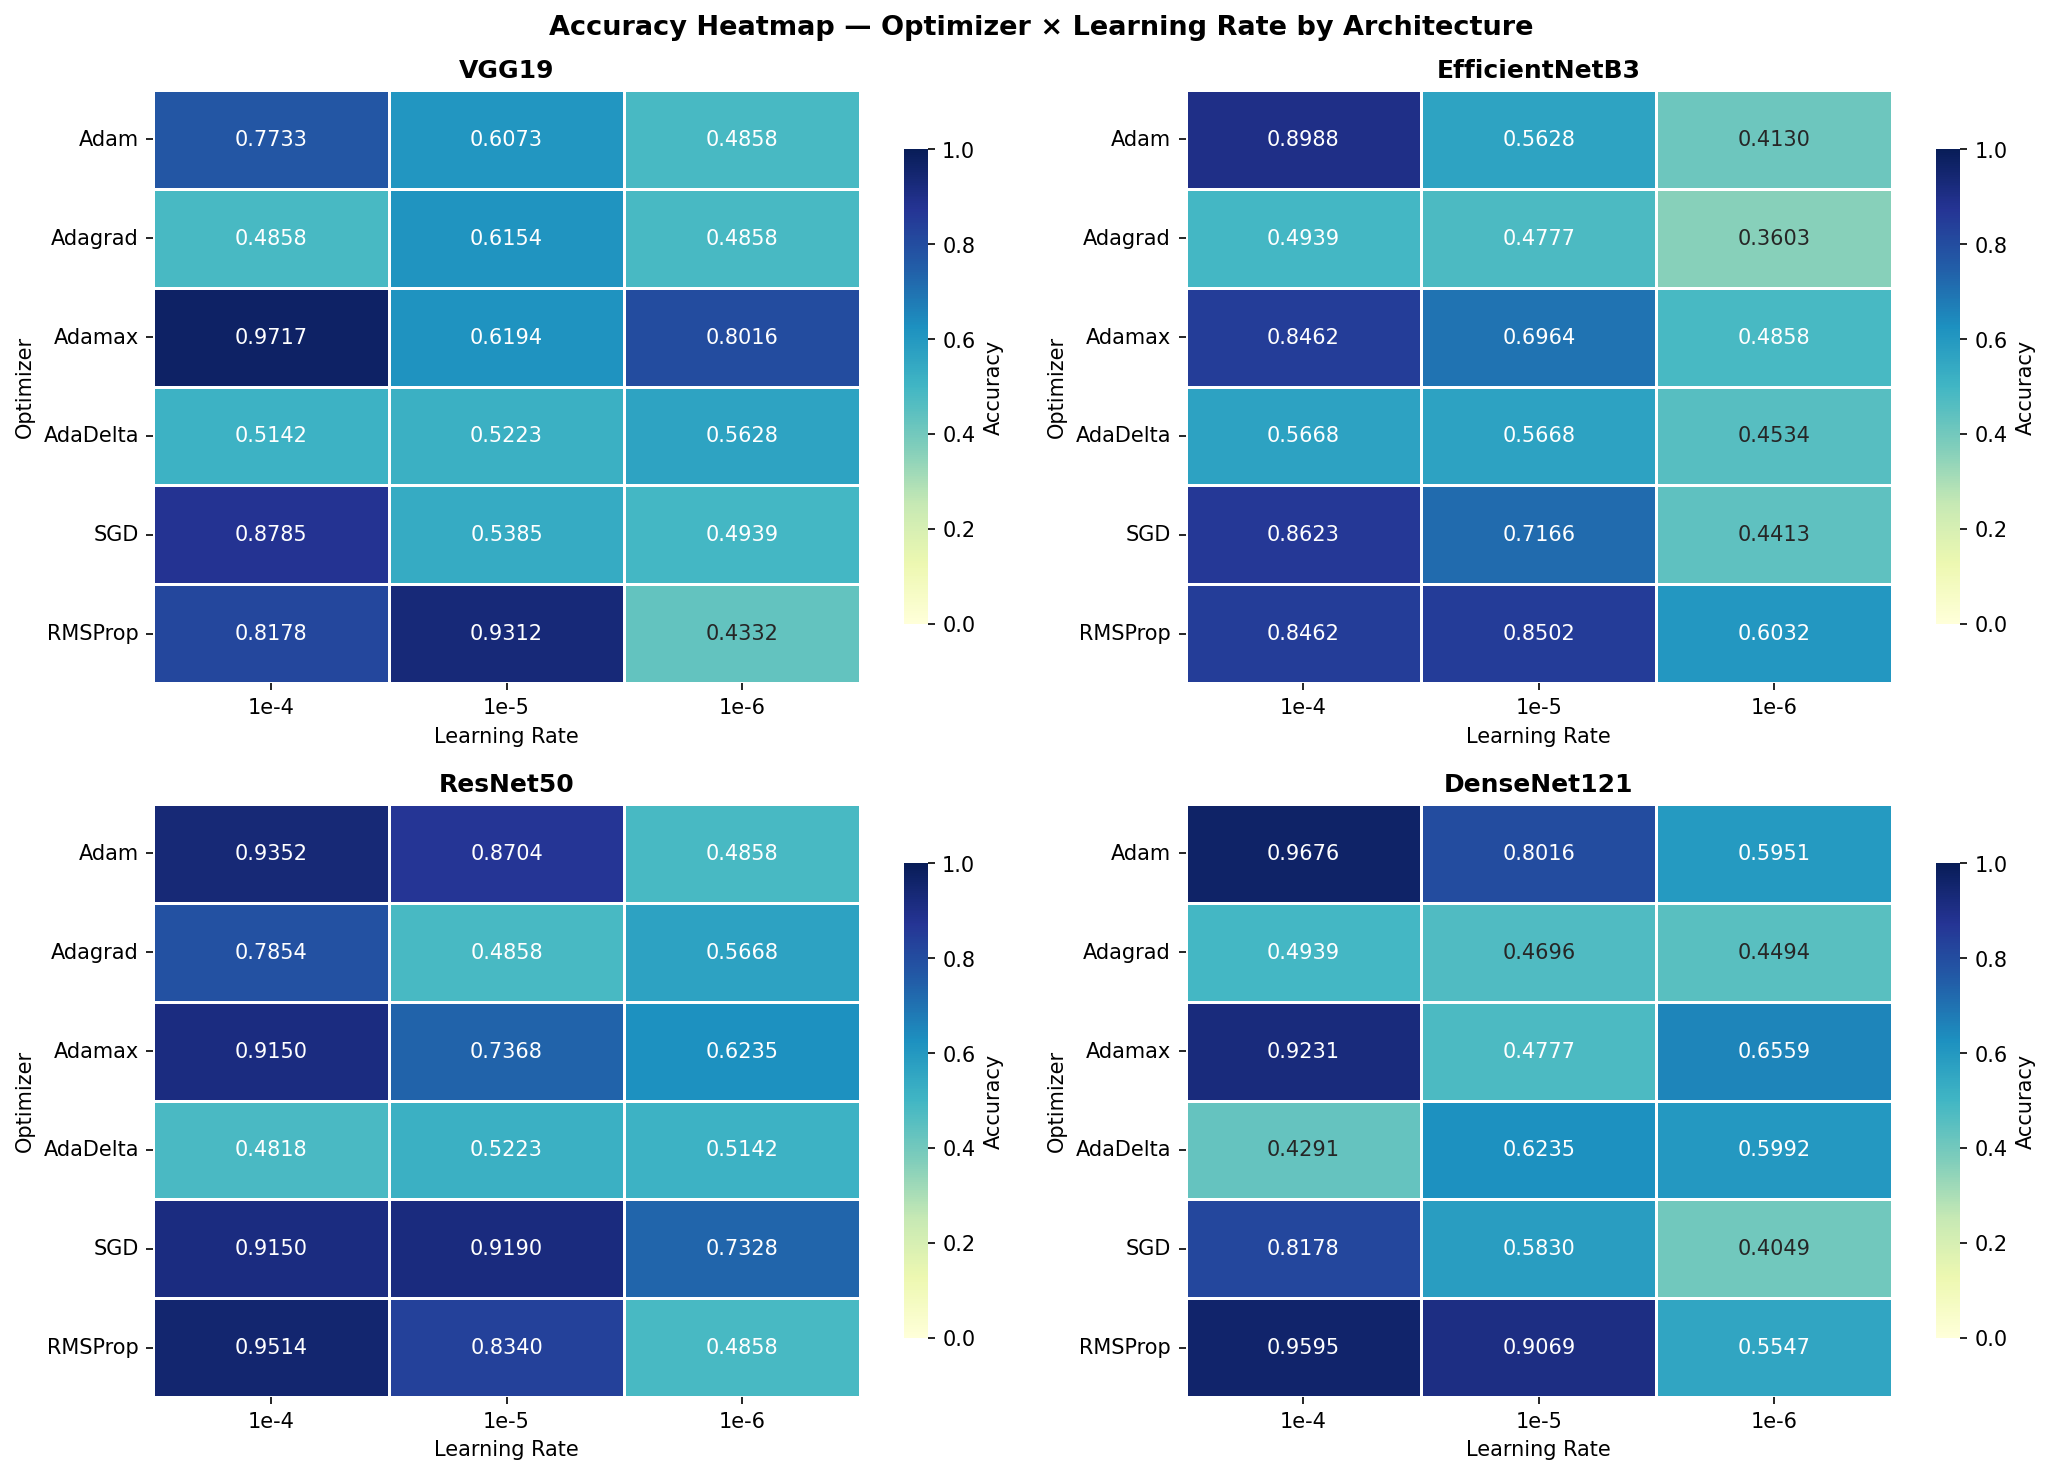
\includegraphics[width=\textwidth]{figures/accuracy_heatmap.png}
  \caption[Full Accuracy Heatmap]{Accuracy across all 72 configurations.}
  \label{fig:heatmap-acc}
\end{figure}

\begin{figure}[htbp]
  \centering
  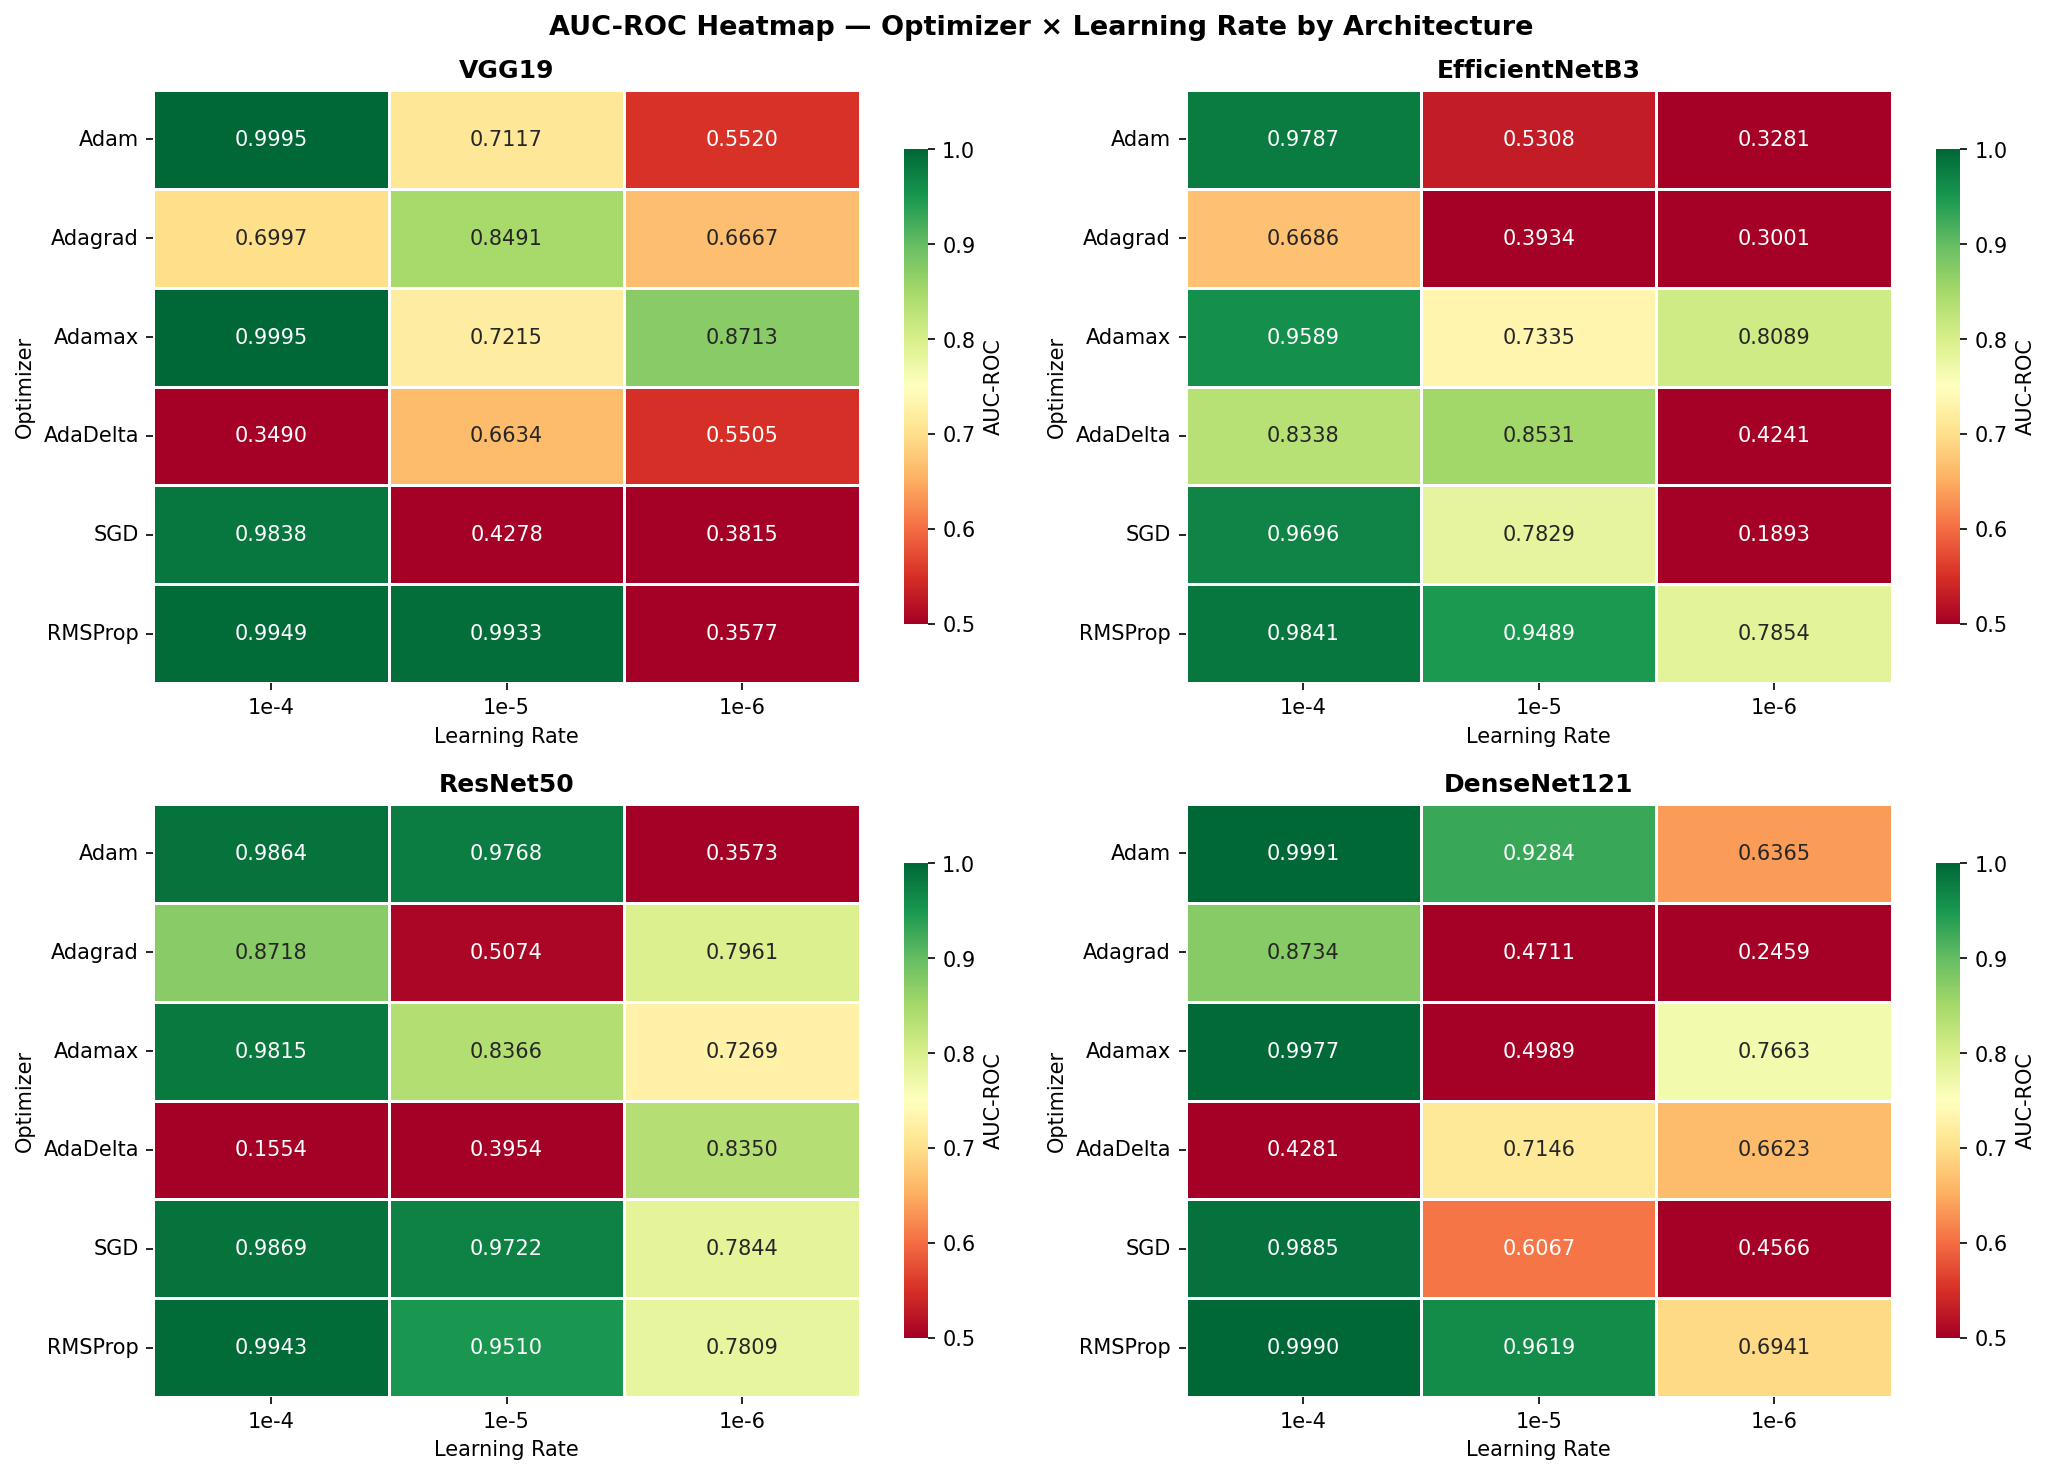
\includegraphics[width=\textwidth]{figures/auc_heatmap.png}
  \caption[Full AUC-ROC Heatmap]{AUC-ROC across all 72 configurations.}
  \label{fig:heatmap-auc}
\end{figure}

\subsection{Failures and Degenerate Runs}

It's also worth noting the runs that failed. We identified 10 cases where the models simply "collapsed" to predicting one class. Interestingly, some of these runs still showed a high AUC (above 0.80) even though they were practically useless because they never correctly identified a single cancer (or non-cancer) case. This highlighted why we need to look at more than just AUC when evaluating these models for medical use.


\newpage
\section{Discussion}
\label{sec:discussion}

\subsection{Why Learning Rate Controlled Everything}

The results show a very clear pattern: the learning rate was the single most important factor in whether a model succeeded or failed. At $10^{-6}$, almost every model struggled. This makes sense when you consider that we kept the base convolutional layers frozen. Since we were starting the classification head from scratch, those weights needed a decent-sized push to start learning the features extracted by the pre-trained model. At $10^{-6}$, the updates were so tiny that the model barely moved from its initial random state before our \texttt{EarlyStopping} callback cut it off.

It is worth noting that early stopping any of the configurations does not confirm whether or not the respective model had finished learning. Note that the callback was set with a patience of 10 epochs and a minimum delta of 0.001 on \texttt{val\_auc}, indicating that the run was halted only when there was no meaningful improvement over 10 consecutive epochs. Within the 72 runs conducted in this study, this limit was set to build consistency amongst the results over seeking out peak performance. Thus, it is worth acknowledging that the results for 1e-6 configurations are representative of the learning rate's performance under the specific conditions of the study as opposed to the upper limit of what those configuraitons were capable of achieving given more time. 
\subsection{Comparing the Optimizers}

A notable observation was how the different optimizers handled the relatively small dataset. RMSProp was the winner here, followed closely by Adam and Adamax. These adaptive methods are great for medical imaging projects like this because they can adjust their updates based on the gradients they see, which helps when the data is limited and potentially noisy.

In contrast, AdaDelta was surprisingly poor. It is meant to be an improvement over Adagrad, but on the provided dataset, it seemed to stall almost immediately. This may be due to, with so few steps per epoch, AdaDelta's internal learning rate calculation dropping to zero before the model could find a good path. 

\subsection{Architecture Strengths}

ResNet50 was the most reliable performer across the arhitecture suite. This may be due to its skip connections helping keep the gradient signal clean as it passes back to the classification head. VGG19 actually rendered the single best individual run, which might be because its simpler, older architecture produces very straightforward features that the pooling-and-dense head could easily interpret. 

EfficientNetB3, which is the most modern model tested, actually came in last on average. Which may be surprising, but it's possible that its more complex feature space needs a lot more data than our 518 training images to really perform to specification.

\subsection{A Warning about AUC}

One of the most important takeaways for us was about the AUC metric itself. We saw several suboptimal runs where the model predicted the same class for every single image, yet they still had an AUC over 0.80. For instance, the VGG19 + Adam (LR=$10^{-6}$) (Figure~\ref{fig:cm-vgg19-adam-lr1e6}) with gradient updates so miniscule, the model weights never meaningully left from start; leading to all 247 test images to be predicted as cancer without exception, an F1 of 0, and a test accuracy of 48.58\% (seemingly random chance) despite a retention of AUC 0.5520. This happens because AUC measures how well the model ranks images, not how well it classifies them at a specific threshold. In a real clinical setting, a model that never finds a single cancer case is a total failure, even if its ranking ability looks good on paper. This reinforces the need to always check recall and specificity alongside AUC.

\subsection{Recommendations}

Should the research be continued, the next logical step would be fine-tuning. We kept the base models frozen to see what a clean transfer learning performance looked like, but unfreezing the last few layers and training them at a very low learning rate would likely boost the scores significantly. It would be prudent to try $k$-fold cross-validation to get a better sense of how these models generalize across different subsets of the data. Furthermore, future efforts are recommended to conduct follow-up simulations with a higher early stopping threshold (e.g. 20 or 30 more epochs), or no early stopping at all. The current simulation setup would not be able to meaningfully distinguish between a configuration that failed to learn anything, and a configuration that was terminated before it was given any meaningful time to learn. Isolating learning rate would further clarify whether the learning rate is reflective of the true upper limits of configuration performance or whether it is an artifact of the stopping criteria. 


\newpage
\section{Conclusion}
\label{sec:conclusion}

In this study, we systematically tested 72 different deep learning configurations to see how they performed at classifying ovarian cancer images. By looking at four different architectures across six optimizers and three learning rates, we have gained a much clearer picture of what works for this kind of medical imaging task.

Our main findings are quite clear:
\begin{itemize}
    \item \textbf{Learning Rate is Key:} For frozen transfer learning on this dataset, a learning rate of $10^{-4}$ is essential. Anything smaller often leads to model collapse.
    \item \textbf{Top Optimizers:} RMSProp, Adam, and Adamax are the most reliable choices for this task.
    \item \textbf{Reliable Models:} ResNet50 was the most consistent overall, while VGG19 produced the single best individual result.
    \item \textbf{Metric Caution:} We can't rely on AUC alone; checking for suboptimal runs using recall and specificity is critical for medical safety.
\end{itemize}

While these results are promising, they are just a starting point. We hope our findings provide a useful baseline for others working on similar medical classification problems, helping them choose the right optimization settings more quickly and avoid common pitfalls like suboptimal convergence.


% ── Appendices ────────────────────────────────────────────────────────────────
\newpage
\section{Appendices}

\subsection{Per-Model Accuracy and Loss Curves}
\label{appx:acc-loss}
% Note: src/visualize.py saves both accuracy/loss curves and AUC-ROC curves to
% {run_dir}/{run_name}.png. In src/train.py, plot_auc_roc() is called after
% plot_accuracy_loss() using the same directory, so the AUC-ROC file overwrites
% the accuracy/loss file. The figures referenced here are the files present on disk
% after training. If accuracy/loss curves are needed separately, re-run training
% with separate output_dir arguments or save plot_accuracy_loss to a curves/ subdirectory.

\clearpage

% ── VGG19 ─────────────────────────────────────────────────────────────────────
\subsection*{VGG19}

\begin{figure}[htbp]
  \centering
  \begin{subfigure}[b]{0.3\textwidth}
    \includegraphics[width=\textwidth]{../../results/VGG19_Adam_LR1e-04/VGG19_Adam_LR1e-04.png}
    \caption{LR=1e-4}
  \end{subfigure}\hfill
  \begin{subfigure}[b]{0.3\textwidth}
    \includegraphics[width=\textwidth]{../../results/VGG19_Adam_LR1e-05/VGG19_Adam_LR1e-05.png}
    \caption{LR=1e-5}
  \end{subfigure}\hfill
  \begin{subfigure}[b]{0.3\textwidth}
    \includegraphics[width=\textwidth]{../../results/VGG19_Adam_LR1e-06/VGG19_Adam_LR1e-06.png}
    \caption{LR=1e-6}
  \end{subfigure}
  \caption{VGG19,Adam: Accuracy and Loss Curves across Learning Rates}
  \label{fig:acc-loss-vgg19-adam}
\end{figure}

\begin{figure}[htbp]
  \centering
  \begin{subfigure}[b]{0.3\textwidth}
    \includegraphics[width=\textwidth]{../../results/VGG19_Adagrad_LR1e-04/VGG19_Adagrad_LR1e-04.png}
    \caption{LR=1e-4}
  \end{subfigure}\hfill
  \begin{subfigure}[b]{0.3\textwidth}
    \includegraphics[width=\textwidth]{../../results/VGG19_Adagrad_LR1e-05/VGG19_Adagrad_LR1e-05.png}
    \caption{LR=1e-5}
  \end{subfigure}\hfill
  \begin{subfigure}[b]{0.3\textwidth}
    \includegraphics[width=\textwidth]{../../results/VGG19_Adagrad_LR1e-06/VGG19_Adagrad_LR1e-06.png}
    \caption{LR=1e-6}
  \end{subfigure}
  \caption{VGG19,Adagrad: Accuracy and Loss Curves across Learning Rates}
  \label{fig:acc-loss-vgg19-adagrad}
\end{figure}

\begin{figure}[htbp]
  \centering
  \begin{subfigure}[b]{0.3\textwidth}
    \includegraphics[width=\textwidth]{../../results/VGG19_Adamax_LR1e-04/VGG19_Adamax_LR1e-04.png}
    \caption{LR=1e-4}
  \end{subfigure}\hfill
  \begin{subfigure}[b]{0.3\textwidth}
    \includegraphics[width=\textwidth]{../../results/VGG19_Adamax_LR1e-05/VGG19_Adamax_LR1e-05.png}
    \caption{LR=1e-5}
  \end{subfigure}\hfill
  \begin{subfigure}[b]{0.3\textwidth}
    \includegraphics[width=\textwidth]{../../results/VGG19_Adamax_LR1e-06/VGG19_Adamax_LR1e-06.png}
    \caption{LR=1e-6}
  \end{subfigure}
  \caption{VGG19,Adamax: Accuracy and Loss Curves across Learning Rates}
  \label{fig:acc-loss-vgg19-adamax}
\end{figure}

\begin{figure}[htbp]
  \centering
  \begin{subfigure}[b]{0.3\textwidth}
    \includegraphics[width=\textwidth]{../../results/VGG19_AdaDelta_LR1e-04/VGG19_AdaDelta_LR1e-04.png}
    \caption{LR=1e-4}
  \end{subfigure}\hfill
  \begin{subfigure}[b]{0.3\textwidth}
    \includegraphics[width=\textwidth]{../../results/VGG19_AdaDelta_LR1e-05/VGG19_AdaDelta_LR1e-05.png}
    \caption{LR=1e-5}
  \end{subfigure}\hfill
  \begin{subfigure}[b]{0.3\textwidth}
    \includegraphics[width=\textwidth]{../../results/VGG19_AdaDelta_LR1e-06/VGG19_AdaDelta_LR1e-06.png}
    \caption{LR=1e-6}
  \end{subfigure}
  \caption{VGG19,AdaDelta: Accuracy and Loss Curves across Learning Rates}
  \label{fig:acc-loss-vgg19-adadelta}
\end{figure}

\begin{figure}[htbp]
  \centering
  \begin{subfigure}[b]{0.3\textwidth}
    \includegraphics[width=\textwidth]{../../results/VGG19_SGD_LR1e-04/VGG19_SGD_LR1e-04.png}
    \caption{LR=1e-4}
  \end{subfigure}\hfill
  \begin{subfigure}[b]{0.3\textwidth}
    \includegraphics[width=\textwidth]{../../results/VGG19_SGD_LR1e-05/VGG19_SGD_LR1e-05.png}
    \caption{LR=1e-5}
  \end{subfigure}\hfill
  \begin{subfigure}[b]{0.3\textwidth}
    \includegraphics[width=\textwidth]{../../results/VGG19_SGD_LR1e-06/VGG19_SGD_LR1e-06.png}
    \caption{LR=1e-6}
  \end{subfigure}
  \caption{VGG19,SGD: Accuracy and Loss Curves across Learning Rates}
  \label{fig:acc-loss-vgg19-sgd}
\end{figure}

\begin{figure}[htbp]
  \centering
  \begin{subfigure}[b]{0.3\textwidth}
    \includegraphics[width=\textwidth]{../../results/VGG19_RMSProp_LR1e-04/VGG19_RMSProp_LR1e-04.png}
    \caption{LR=1e-4}
  \end{subfigure}\hfill
  \begin{subfigure}[b]{0.3\textwidth}
    \includegraphics[width=\textwidth]{../../results/VGG19_RMSProp_LR1e-05/VGG19_RMSProp_LR1e-05.png}
    \caption{LR=1e-5}
  \end{subfigure}\hfill
  \begin{subfigure}[b]{0.3\textwidth}
    \includegraphics[width=\textwidth]{../../results/VGG19_RMSProp_LR1e-06/VGG19_RMSProp_LR1e-06.png}
    \caption{LR=1e-6}
  \end{subfigure}
  \caption{VGG19,RMSProp: Accuracy and Loss Curves across Learning Rates}
  \label{fig:acc-loss-vgg19-rmsprop}
\end{figure}

\begin{figure}[htbp]
  \centering
  \begin{subfigure}[b]{0.3\textwidth}
    \includegraphics[width=\textwidth]{../../results/VGG19_Nadam_LR1e-04/VGG19_Nadam_LR1e-04.png}
    \caption{LR=1e-4}
  \end{subfigure}\hfill
  \begin{subfigure}[b]{0.3\textwidth}
    \includegraphics[width=\textwidth]{../../results/VGG19_Nadam_LR1e-05/VGG19_Nadam_LR1e-05.png}
    \caption{LR=1e-5}
  \end{subfigure}\hfill
  \begin{subfigure}[b]{0.3\textwidth}
    \includegraphics[width=\textwidth]{../../results/VGG19_Nadam_LR1e-06/VGG19_Nadam_LR1e-06.png}
    \caption{LR=1e-6}
  \end{subfigure}
  \caption{VGG19,Nadam: Accuracy and Loss Curves across Learning Rates}
  \label{fig:acc-loss-vgg19-nadam}
\end{figure}

\clearpage

% ── EfficientNetB3 ────────────────────────────────────────────────────────────
\subsection*{EfficientNetB3}

\begin{figure}[htbp]
  \centering
  \begin{subfigure}[b]{0.3\textwidth}
    \includegraphics[width=\textwidth]{../../results/EfficientNetB3_Adam_LR1e-04/EfficientNetB3_Adam_LR1e-04.png}
    \caption{LR=1e-4}
  \end{subfigure}\hfill
  \begin{subfigure}[b]{0.3\textwidth}
    \includegraphics[width=\textwidth]{../../results/EfficientNetB3_Adam_LR1e-05/EfficientNetB3_Adam_LR1e-05.png}
    \caption{LR=1e-5}
  \end{subfigure}\hfill
  \begin{subfigure}[b]{0.3\textwidth}
    \includegraphics[width=\textwidth]{../../results/EfficientNetB3_Adam_LR1e-06/EfficientNetB3_Adam_LR1e-06.png}
    \caption{LR=1e-6}
  \end{subfigure}
  \caption{EfficientNetB3,Adam: Accuracy and Loss Curves across Learning Rates}
  \label{fig:acc-loss-effnet-adam}
\end{figure}

\begin{figure}[htbp]
  \centering
  \begin{subfigure}[b]{0.3\textwidth}
    \includegraphics[width=\textwidth]{../../results/EfficientNetB3_Adagrad_LR1e-04/EfficientNetB3_Adagrad_LR1e-04.png}
    \caption{LR=1e-4}
  \end{subfigure}\hfill
  \begin{subfigure}[b]{0.3\textwidth}
    \includegraphics[width=\textwidth]{../../results/EfficientNetB3_Adagrad_LR1e-05/EfficientNetB3_Adagrad_LR1e-05.png}
    \caption{LR=1e-5}
  \end{subfigure}\hfill
  \begin{subfigure}[b]{0.3\textwidth}
    \includegraphics[width=\textwidth]{../../results/EfficientNetB3_Adagrad_LR1e-06/EfficientNetB3_Adagrad_LR1e-06.png}
    \caption{LR=1e-6}
  \end{subfigure}
  \caption{EfficientNetB3,Adagrad: Accuracy and Loss Curves across Learning Rates}
  \label{fig:acc-loss-effnet-adagrad}
\end{figure}

\begin{figure}[htbp]
  \centering
  \begin{subfigure}[b]{0.3\textwidth}
    \includegraphics[width=\textwidth]{../../results/EfficientNetB3_Adamax_LR1e-04/EfficientNetB3_Adamax_LR1e-04.png}
    \caption{LR=1e-4}
  \end{subfigure}\hfill
  \begin{subfigure}[b]{0.3\textwidth}
    \includegraphics[width=\textwidth]{../../results/EfficientNetB3_Adamax_LR1e-05/EfficientNetB3_Adamax_LR1e-05.png}
    \caption{LR=1e-5}
  \end{subfigure}\hfill
  \begin{subfigure}[b]{0.3\textwidth}
    \includegraphics[width=\textwidth]{../../results/EfficientNetB3_Adamax_LR1e-06/EfficientNetB3_Adamax_LR1e-06.png}
    \caption{LR=1e-6}
  \end{subfigure}
  \caption{EfficientNetB3,Adamax: Accuracy and Loss Curves across Learning Rates}
  \label{fig:acc-loss-effnet-adamax}
\end{figure}

\begin{figure}[htbp]
  \centering
  \begin{subfigure}[b]{0.3\textwidth}
    \includegraphics[width=\textwidth]{../../results/EfficientNetB3_AdaDelta_LR1e-04/EfficientNetB3_AdaDelta_LR1e-04.png}
    \caption{LR=1e-4}
  \end{subfigure}\hfill
  \begin{subfigure}[b]{0.3\textwidth}
    \includegraphics[width=\textwidth]{../../results/EfficientNetB3_AdaDelta_LR1e-05/EfficientNetB3_AdaDelta_LR1e-05.png}
    \caption{LR=1e-5}
  \end{subfigure}\hfill
  \begin{subfigure}[b]{0.3\textwidth}
    \includegraphics[width=\textwidth]{../../results/EfficientNetB3_AdaDelta_LR1e-06/EfficientNetB3_AdaDelta_LR1e-06.png}
    \caption{LR=1e-6}
  \end{subfigure}
  \caption{EfficientNetB3,AdaDelta: Accuracy and Loss Curves across Learning Rates}
  \label{fig:acc-loss-effnet-adadelta}
\end{figure}

\begin{figure}[htbp]
  \centering
  \begin{subfigure}[b]{0.3\textwidth}
    \includegraphics[width=\textwidth]{../../results/EfficientNetB3_SGD_LR1e-04/EfficientNetB3_SGD_LR1e-04.png}
    \caption{LR=1e-4}
  \end{subfigure}\hfill
  \begin{subfigure}[b]{0.3\textwidth}
    \includegraphics[width=\textwidth]{../../results/EfficientNetB3_SGD_LR1e-05/EfficientNetB3_SGD_LR1e-05.png}
    \caption{LR=1e-5}
  \end{subfigure}\hfill
  \begin{subfigure}[b]{0.3\textwidth}
    \includegraphics[width=\textwidth]{../../results/EfficientNetB3_SGD_LR1e-06/EfficientNetB3_SGD_LR1e-06.png}
    \caption{LR=1e-6}
  \end{subfigure}
  \caption{EfficientNetB3,SGD: Accuracy and Loss Curves across Learning Rates}
  \label{fig:acc-loss-effnet-sgd}
\end{figure}

\begin{figure}[htbp]
  \centering
  \begin{subfigure}[b]{0.3\textwidth}
    \includegraphics[width=\textwidth]{../../results/EfficientNetB3_RMSProp_LR1e-04/EfficientNetB3_RMSProp_LR1e-04.png}
    \caption{LR=1e-4}
  \end{subfigure}\hfill
  \begin{subfigure}[b]{0.3\textwidth}
    \includegraphics[width=\textwidth]{../../results/EfficientNetB3_RMSProp_LR1e-05/EfficientNetB3_RMSProp_LR1e-05.png}
    \caption{LR=1e-5}
  \end{subfigure}\hfill
  \begin{subfigure}[b]{0.3\textwidth}
    \includegraphics[width=\textwidth]{../../results/EfficientNetB3_RMSProp_LR1e-06/EfficientNetB3_RMSProp_LR1e-06.png}
    \caption{LR=1e-6}
  \end{subfigure}
  \caption{EfficientNetB3,RMSProp: Accuracy and Loss Curves across Learning Rates}
  \label{fig:acc-loss-effnet-rmsprop}
\end{figure}

\begin{figure}[htbp]
  \centering
  \begin{subfigure}[b]{0.3\textwidth}
    \includegraphics[width=\textwidth]{../../results/EfficientNetB3_Nadam_LR1e-04/EfficientNetB3_Nadam_LR1e-04.png}
    \caption{LR=1e-4}
  \end{subfigure}\hfill
  \begin{subfigure}[b]{0.3\textwidth}
    \includegraphics[width=\textwidth]{../../results/EfficientNetB3_Nadam_LR1e-05/EfficientNetB3_Nadam_LR1e-05.png}
    \caption{LR=1e-5}
  \end{subfigure}\hfill
  \begin{subfigure}[b]{0.3\textwidth}
    \includegraphics[width=\textwidth]{../../results/EfficientNetB3_Nadam_LR1e-06/EfficientNetB3_Nadam_LR1e-06.png}
    \caption{LR=1e-6}
  \end{subfigure}
  \caption{EfficientNetB3,Nadam: Accuracy and Loss Curves across Learning Rates}
  \label{fig:acc-loss-effnet-nadam}
\end{figure}

\clearpage

% ── ResNet50 ──────────────────────────────────────────────────────────────────
\subsection*{ResNet50}

\begin{figure}[htbp]
  \centering
  \begin{subfigure}[b]{0.3\textwidth}
    \includegraphics[width=\textwidth]{../../results/ResNet50_Adam_LR1e-04/ResNet50_Adam_LR1e-04.png}
    \caption{LR=1e-4}
  \end{subfigure}\hfill
  \begin{subfigure}[b]{0.3\textwidth}
    \includegraphics[width=\textwidth]{../../results/ResNet50_Adam_LR1e-05/ResNet50_Adam_LR1e-05.png}
    \caption{LR=1e-5}
  \end{subfigure}\hfill
  \begin{subfigure}[b]{0.3\textwidth}
    \includegraphics[width=\textwidth]{../../results/ResNet50_Adam_LR1e-06/ResNet50_Adam_LR1e-06.png}
    \caption{LR=1e-6}
  \end{subfigure}
  \caption{ResNet50,Adam: Accuracy and Loss Curves across Learning Rates}
  \label{fig:acc-loss-resnet-adam}
\end{figure}

\begin{figure}[htbp]
  \centering
  \begin{subfigure}[b]{0.3\textwidth}
    \includegraphics[width=\textwidth]{../../results/ResNet50_Adagrad_LR1e-04/ResNet50_Adagrad_LR1e-04.png}
    \caption{LR=1e-4}
  \end{subfigure}\hfill
  \begin{subfigure}[b]{0.3\textwidth}
    \includegraphics[width=\textwidth]{../../results/ResNet50_Adagrad_LR1e-05/ResNet50_Adagrad_LR1e-05.png}
    \caption{LR=1e-5}
  \end{subfigure}\hfill
  \begin{subfigure}[b]{0.3\textwidth}
    \includegraphics[width=\textwidth]{../../results/ResNet50_Adagrad_LR1e-06/ResNet50_Adagrad_LR1e-06.png}
    \caption{LR=1e-6}
  \end{subfigure}
  \caption{ResNet50,Adagrad: Accuracy and Loss Curves across Learning Rates}
  \label{fig:acc-loss-resnet-adagrad}
\end{figure}

\begin{figure}[htbp]
  \centering
  \begin{subfigure}[b]{0.3\textwidth}
    \includegraphics[width=\textwidth]{../../results/ResNet50_Adamax_LR1e-04/ResNet50_Adamax_LR1e-04.png}
    \caption{LR=1e-4}
  \end{subfigure}\hfill
  \begin{subfigure}[b]{0.3\textwidth}
    \includegraphics[width=\textwidth]{../../results/ResNet50_Adamax_LR1e-05/ResNet50_Adamax_LR1e-05.png}
    \caption{LR=1e-5}
  \end{subfigure}\hfill
  \begin{subfigure}[b]{0.3\textwidth}
    \includegraphics[width=\textwidth]{../../results/ResNet50_Adamax_LR1e-06/ResNet50_Adamax_LR1e-06.png}
    \caption{LR=1e-6}
  \end{subfigure}
  \caption{ResNet50,Adamax: Accuracy and Loss Curves across Learning Rates}
  \label{fig:acc-loss-resnet-adamax}
\end{figure}

\begin{figure}[htbp]
  \centering
  \begin{subfigure}[b]{0.3\textwidth}
    \includegraphics[width=\textwidth]{../../results/ResNet50_AdaDelta_LR1e-04/ResNet50_AdaDelta_LR1e-04.png}
    \caption{LR=1e-4}
  \end{subfigure}\hfill
  \begin{subfigure}[b]{0.3\textwidth}
    \includegraphics[width=\textwidth]{../../results/ResNet50_AdaDelta_LR1e-05/ResNet50_AdaDelta_LR1e-05.png}
    \caption{LR=1e-5}
  \end{subfigure}\hfill
  \begin{subfigure}[b]{0.3\textwidth}
    \includegraphics[width=\textwidth]{../../results/ResNet50_AdaDelta_LR1e-06/ResNet50_AdaDelta_LR1e-06.png}
    \caption{LR=1e-6}
  \end{subfigure}
  \caption{ResNet50,AdaDelta: Accuracy and Loss Curves across Learning Rates}
  \label{fig:acc-loss-resnet-adadelta}
\end{figure}

\begin{figure}[htbp]
  \centering
  \begin{subfigure}[b]{0.3\textwidth}
    \includegraphics[width=\textwidth]{../../results/ResNet50_SGD_LR1e-04/ResNet50_SGD_LR1e-04.png}
    \caption{LR=1e-4}
  \end{subfigure}\hfill
  \begin{subfigure}[b]{0.3\textwidth}
    \includegraphics[width=\textwidth]{../../results/ResNet50_SGD_LR1e-05/ResNet50_SGD_LR1e-05.png}
    \caption{LR=1e-5}
  \end{subfigure}\hfill
  \begin{subfigure}[b]{0.3\textwidth}
    \includegraphics[width=\textwidth]{../../results/ResNet50_SGD_LR1e-06/ResNet50_SGD_LR1e-06.png}
    \caption{LR=1e-6}
  \end{subfigure}
  \caption{ResNet50,SGD: Accuracy and Loss Curves across Learning Rates}
  \label{fig:acc-loss-resnet-sgd}
\end{figure}

\begin{figure}[htbp]
  \centering
  \begin{subfigure}[b]{0.3\textwidth}
    \includegraphics[width=\textwidth]{../../results/ResNet50_RMSProp_LR1e-04/ResNet50_RMSProp_LR1e-04.png}
    \caption{LR=1e-4}
  \end{subfigure}\hfill
  \begin{subfigure}[b]{0.3\textwidth}
    \includegraphics[width=\textwidth]{../../results/ResNet50_RMSProp_LR1e-05/ResNet50_RMSProp_LR1e-05.png}
    \caption{LR=1e-5}
  \end{subfigure}\hfill
  \begin{subfigure}[b]{0.3\textwidth}
    \includegraphics[width=\textwidth]{../../results/ResNet50_RMSProp_LR1e-06/ResNet50_RMSProp_LR1e-06.png}
    \caption{LR=1e-6}
  \end{subfigure}
  \caption{ResNet50,RMSProp: Accuracy and Loss Curves across Learning Rates}
  \label{fig:acc-loss-resnet-rmsprop}
\end{figure}

\begin{figure}[htbp]
  \centering
  \begin{subfigure}[b]{0.3\textwidth}
    \includegraphics[width=\textwidth]{../../results/ResNet50_Nadam_LR1e-04/ResNet50_Nadam_LR1e-04.png}
    \caption{LR=1e-4}
  \end{subfigure}\hfill
  \begin{subfigure}[b]{0.3\textwidth}
    \includegraphics[width=\textwidth]{../../results/ResNet50_Nadam_LR1e-05/ResNet50_Nadam_LR1e-05.png}
    \caption{LR=1e-5}
  \end{subfigure}\hfill
  \begin{subfigure}[b]{0.3\textwidth}
    \includegraphics[width=\textwidth]{../../results/ResNet50_Nadam_LR1e-06/ResNet50_Nadam_LR1e-06.png}
    \caption{LR=1e-6}
  \end{subfigure}
  \caption{ResNet50,Nadam: Accuracy and Loss Curves across Learning Rates}
  \label{fig:acc-loss-resnet-nadam}
\end{figure}

\clearpage

% ── DenseNet121 ───────────────────────────────────────────────────────────────
\subsection*{DenseNet121}

\begin{figure}[htbp]
  \centering
  \begin{subfigure}[b]{0.3\textwidth}
    \includegraphics[width=\textwidth]{../../results/DenseNet121_Adam_LR1e-04/DenseNet121_Adam_LR1e-04.png}
    \caption{LR=1e-4}
  \end{subfigure}\hfill
  \begin{subfigure}[b]{0.3\textwidth}
    \includegraphics[width=\textwidth]{../../results/DenseNet121_Adam_LR1e-05/DenseNet121_Adam_LR1e-05.png}
    \caption{LR=1e-5}
  \end{subfigure}\hfill
  \begin{subfigure}[b]{0.3\textwidth}
    \includegraphics[width=\textwidth]{../../results/DenseNet121_Adam_LR1e-06/DenseNet121_Adam_LR1e-06.png}
    \caption{LR=1e-6}
  \end{subfigure}
  \caption{DenseNet121,Adam: Accuracy and Loss Curves across Learning Rates}
  \label{fig:acc-loss-densenet-adam}
\end{figure}

\begin{figure}[htbp]
  \centering
  \begin{subfigure}[b]{0.3\textwidth}
    \includegraphics[width=\textwidth]{../../results/DenseNet121_Adagrad_LR1e-04/DenseNet121_Adagrad_LR1e-04.png}
    \caption{LR=1e-4}
  \end{subfigure}\hfill
  \begin{subfigure}[b]{0.3\textwidth}
    \includegraphics[width=\textwidth]{../../results/DenseNet121_Adagrad_LR1e-05/DenseNet121_Adagrad_LR1e-05.png}
    \caption{LR=1e-5}
  \end{subfigure}\hfill
  \begin{subfigure}[b]{0.3\textwidth}
    \includegraphics[width=\textwidth]{../../results/DenseNet121_Adagrad_LR1e-06/DenseNet121_Adagrad_LR1e-06.png}
    \caption{LR=1e-6}
  \end{subfigure}
  \caption{DenseNet121,Adagrad: Accuracy and Loss Curves across Learning Rates}
  \label{fig:acc-loss-densenet-adagrad}
\end{figure}

\begin{figure}[htbp]
  \centering
  \begin{subfigure}[b]{0.3\textwidth}
    \includegraphics[width=\textwidth]{../../results/DenseNet121_Adamax_LR1e-04/DenseNet121_Adamax_LR1e-04.png}
    \caption{LR=1e-4}
  \end{subfigure}\hfill
  \begin{subfigure}[b]{0.3\textwidth}
    \includegraphics[width=\textwidth]{../../results/DenseNet121_Adamax_LR1e-05/DenseNet121_Adamax_LR1e-05.png}
    \caption{LR=1e-5}
  \end{subfigure}\hfill
  \begin{subfigure}[b]{0.3\textwidth}
    \includegraphics[width=\textwidth]{../../results/DenseNet121_Adamax_LR1e-06/DenseNet121_Adamax_LR1e-06.png}
    \caption{LR=1e-6}
  \end{subfigure}
  \caption{DenseNet121,Adamax: Accuracy and Loss Curves across Learning Rates}
  \label{fig:acc-loss-densenet-adamax}
\end{figure}

\begin{figure}[htbp]
  \centering
  \begin{subfigure}[b]{0.3\textwidth}
    \includegraphics[width=\textwidth]{../../results/DenseNet121_AdaDelta_LR1e-04/DenseNet121_AdaDelta_LR1e-04.png}
    \caption{LR=1e-4}
  \end{subfigure}\hfill
  \begin{subfigure}[b]{0.3\textwidth}
    \includegraphics[width=\textwidth]{../../results/DenseNet121_AdaDelta_LR1e-05/DenseNet121_AdaDelta_LR1e-05.png}
    \caption{LR=1e-5}
  \end{subfigure}\hfill
  \begin{subfigure}[b]{0.3\textwidth}
    \includegraphics[width=\textwidth]{../../results/DenseNet121_AdaDelta_LR1e-06/DenseNet121_AdaDelta_LR1e-06.png}
    \caption{LR=1e-6}
  \end{subfigure}
  \caption{DenseNet121,AdaDelta: Accuracy and Loss Curves across Learning Rates}
  \label{fig:acc-loss-densenet-adadelta}
\end{figure}

\begin{figure}[htbp]
  \centering
  \begin{subfigure}[b]{0.3\textwidth}
    \includegraphics[width=\textwidth]{../../results/DenseNet121_SGD_LR1e-04/DenseNet121_SGD_LR1e-04.png}
    \caption{LR=1e-4}
  \end{subfigure}\hfill
  \begin{subfigure}[b]{0.3\textwidth}
    \includegraphics[width=\textwidth]{../../results/DenseNet121_SGD_LR1e-05/DenseNet121_SGD_LR1e-05.png}
    \caption{LR=1e-5}
  \end{subfigure}\hfill
  \begin{subfigure}[b]{0.3\textwidth}
    \includegraphics[width=\textwidth]{../../results/DenseNet121_SGD_LR1e-06/DenseNet121_SGD_LR1e-06.png}
    \caption{LR=1e-6}
  \end{subfigure}
  \caption{DenseNet121,SGD: Accuracy and Loss Curves across Learning Rates}
  \label{fig:acc-loss-densenet-sgd}
\end{figure}

\begin{figure}[htbp]
  \centering
  \begin{subfigure}[b]{0.3\textwidth}
    \includegraphics[width=\textwidth]{../../results/DenseNet121_RMSProp_LR1e-04/DenseNet121_RMSProp_LR1e-04.png}
    \caption{LR=1e-4}
  \end{subfigure}\hfill
  \begin{subfigure}[b]{0.3\textwidth}
    \includegraphics[width=\textwidth]{../../results/DenseNet121_RMSProp_LR1e-05/DenseNet121_RMSProp_LR1e-05.png}
    \caption{LR=1e-5}
  \end{subfigure}\hfill
  \begin{subfigure}[b]{0.3\textwidth}
    \includegraphics[width=\textwidth]{../../results/DenseNet121_RMSProp_LR1e-06/DenseNet121_RMSProp_LR1e-06.png}
    \caption{LR=1e-6}
  \end{subfigure}
  \caption{DenseNet121,RMSProp: Accuracy and Loss Curves across Learning Rates}
  \label{fig:acc-loss-densenet-rmsprop}
\end{figure}

\begin{figure}[htbp]
  \centering
  \begin{subfigure}[b]{0.3\textwidth}
    \includegraphics[width=\textwidth]{../../results/DenseNet121_Nadam_LR1e-04/DenseNet121_Nadam_LR1e-04.png}
    \caption{LR=1e-4}
  \end{subfigure}\hfill
  \begin{subfigure}[b]{0.3\textwidth}
    \includegraphics[width=\textwidth]{../../results/DenseNet121_Nadam_LR1e-05/DenseNet121_Nadam_LR1e-05.png}
    \caption{LR=1e-5}
  \end{subfigure}\hfill
  \begin{subfigure}[b]{0.3\textwidth}
    \includegraphics[width=\textwidth]{../../results/DenseNet121_Nadam_LR1e-06/DenseNet121_Nadam_LR1e-06.png}
    \caption{LR=1e-6}
  \end{subfigure}
  \caption{DenseNet121,Nadam: Accuracy and Loss Curves across Learning Rates}
  \label{fig:acc-loss-densenet-nadam}
\end{figure}

\clearpage


\subsection{Per-Model AUC-ROC Curves}
\label{appx:auc-roc}
% AUC-ROC curve files share the same path as accuracy/loss curves:
% src/visualize.py saves both to {run_dir}/{run_name}.png, and in src/train.py
% plot_auc_roc() is called after plot_accuracy_loss(), so the AUC-ROC figure
% is the file present on disk at that path after training completes.

\clearpage

% ── VGG19 ─────────────────────────────────────────────────────────────────────
\begin{figure}[p]
  \centering
  \begin{subfigure}[b]{0.3\textwidth}
    \includegraphics[width=\textwidth]{../../results/VGG19_Adam_LR1e-04/VGG19_Adam_LR1e-04.png}
    \caption{Adam, LR=1e-4}
  \end{subfigure}\hfill
  \begin{subfigure}[b]{0.3\textwidth}
    \includegraphics[width=\textwidth]{../../results/VGG19_Adam_LR1e-05/VGG19_Adam_LR1e-05.png}
    \caption{Adam, LR=1e-5}
  \end{subfigure}\hfill
  \begin{subfigure}[b]{0.3\textwidth}
    \includegraphics[width=\textwidth]{../../results/VGG19_Adam_LR1e-06/VGG19_Adam_LR1e-06.png}
    \caption{Adam, LR=1e-6}
  \end{subfigure}\\[0.3em]
  \begin{subfigure}[b]{0.3\textwidth}
    \includegraphics[width=\textwidth]{../../results/VGG19_Adagrad_LR1e-04/VGG19_Adagrad_LR1e-04.png}
    \caption{Adagrad, LR=1e-4}
  \end{subfigure}\hfill
  \begin{subfigure}[b]{0.3\textwidth}
    \includegraphics[width=\textwidth]{../../results/VGG19_Adagrad_LR1e-05/VGG19_Adagrad_LR1e-05.png}
    \caption{Adagrad, LR=1e-5}
  \end{subfigure}\hfill
  \begin{subfigure}[b]{0.3\textwidth}
    \includegraphics[width=\textwidth]{../../results/VGG19_Adagrad_LR1e-06/VGG19_Adagrad_LR1e-06.png}
    \caption{Adagrad, LR=1e-6}
  \end{subfigure}\\[0.3em]
  \begin{subfigure}[b]{0.3\textwidth}
    \includegraphics[width=\textwidth]{../../results/VGG19_Adamax_LR1e-04/VGG19_Adamax_LR1e-04.png}
    \caption{Adamax, LR=1e-4}
  \end{subfigure}\hfill
  \begin{subfigure}[b]{0.3\textwidth}
    \includegraphics[width=\textwidth]{../../results/VGG19_Adamax_LR1e-05/VGG19_Adamax_LR1e-05.png}
    \caption{Adamax, LR=1e-5}
  \end{subfigure}\hfill
  \begin{subfigure}[b]{0.3\textwidth}
    \includegraphics[width=\textwidth]{../../results/VGG19_Adamax_LR1e-06/VGG19_Adamax_LR1e-06.png}
    \caption{Adamax, LR=1e-6}
  \end{subfigure}\\[0.3em]
  \begin{subfigure}[b]{0.3\textwidth}
    \includegraphics[width=\textwidth]{../../results/VGG19_AdaDelta_LR1e-04/VGG19_AdaDelta_LR1e-04.png}
    \caption{AdaDelta, LR=1e-4}
  \end{subfigure}\hfill
  \begin{subfigure}[b]{0.3\textwidth}
    \includegraphics[width=\textwidth]{../../results/VGG19_AdaDelta_LR1e-05/VGG19_AdaDelta_LR1e-05.png}
    \caption{AdaDelta, LR=1e-5}
  \end{subfigure}\hfill
  \begin{subfigure}[b]{0.3\textwidth}
    \includegraphics[width=\textwidth]{../../results/VGG19_AdaDelta_LR1e-06/VGG19_AdaDelta_LR1e-06.png}
    \caption{AdaDelta, LR=1e-6}
  \end{subfigure}\\[0.3em]
  \begin{subfigure}[b]{0.3\textwidth}
    \includegraphics[width=\textwidth]{../../results/VGG19_SGD_LR1e-04/VGG19_SGD_LR1e-04.png}
    \caption{SGD, LR=1e-4}
  \end{subfigure}\hfill
  \begin{subfigure}[b]{0.3\textwidth}
    \includegraphics[width=\textwidth]{../../results/VGG19_SGD_LR1e-05/VGG19_SGD_LR1e-05.png}
    \caption{SGD, LR=1e-5}
  \end{subfigure}\hfill
  \begin{subfigure}[b]{0.3\textwidth}
    \includegraphics[width=\textwidth]{../../results/VGG19_SGD_LR1e-06/VGG19_SGD_LR1e-06.png}
    \caption{SGD, LR=1e-6}
  \end{subfigure}\\[0.3em]
  \begin{subfigure}[b]{0.3\textwidth}
    \includegraphics[width=\textwidth]{../../results/VGG19_RMSProp_LR1e-04/VGG19_RMSProp_LR1e-04.png}
    \caption{RMSProp, LR=1e-4}
  \end{subfigure}\hfill
  \begin{subfigure}[b]{0.3\textwidth}
    \includegraphics[width=\textwidth]{../../results/VGG19_RMSProp_LR1e-05/VGG19_RMSProp_LR1e-05.png}
    \caption{RMSProp, LR=1e-5}
  \end{subfigure}\hfill
  \begin{subfigure}[b]{0.3\textwidth}
    \includegraphics[width=\textwidth]{../../results/VGG19_RMSProp_LR1e-06/VGG19_RMSProp_LR1e-06.png}
    \caption{RMSProp, LR=1e-6}
  \end{subfigure}\\[0.3em]
  \begin{subfigure}[b]{0.3\textwidth}
    \includegraphics[width=\textwidth]{../../results/VGG19_Nadam_LR1e-04/VGG19_Nadam_LR1e-04.png}
    \caption{Nadam, LR=1e-4}
  \end{subfigure}\hfill
  \begin{subfigure}[b]{0.3\textwidth}
    \includegraphics[width=\textwidth]{../../results/VGG19_Nadam_LR1e-05/VGG19_Nadam_LR1e-05.png}
    \caption{Nadam, LR=1e-5}
  \end{subfigure}\hfill
  \begin{subfigure}[b]{0.3\textwidth}
    \includegraphics[width=\textwidth]{../../results/VGG19_Nadam_LR1e-06/VGG19_Nadam_LR1e-06.png}
    \caption{Nadam, LR=1e-6}
  \end{subfigure}
  \caption{AUC-ROC Curves: VGG19 (all 21 configurations).}
  \label{fig:auc-roc-vgg19}
\end{figure}
\clearpage

% ── EfficientNetB3 ────────────────────────────────────────────────────────────
\begin{figure}[p]
  \centering
  \begin{subfigure}[b]{0.3\textwidth}
    \includegraphics[width=\textwidth]{../../results/EfficientNetB3_Adam_LR1e-04/EfficientNetB3_Adam_LR1e-04.png}
    \caption{Adam, LR=1e-4}
  \end{subfigure}\hfill
  \begin{subfigure}[b]{0.3\textwidth}
    \includegraphics[width=\textwidth]{../../results/EfficientNetB3_Adam_LR1e-05/EfficientNetB3_Adam_LR1e-05.png}
    \caption{Adam, LR=1e-5}
  \end{subfigure}\hfill
  \begin{subfigure}[b]{0.3\textwidth}
    \includegraphics[width=\textwidth]{../../results/EfficientNetB3_Adam_LR1e-06/EfficientNetB3_Adam_LR1e-06.png}
    \caption{Adam, LR=1e-6}
  \end{subfigure}\\[0.3em]
  \begin{subfigure}[b]{0.3\textwidth}
    \includegraphics[width=\textwidth]{../../results/EfficientNetB3_Adagrad_LR1e-04/EfficientNetB3_Adagrad_LR1e-04.png}
    \caption{Adagrad, LR=1e-4}
  \end{subfigure}\hfill
  \begin{subfigure}[b]{0.3\textwidth}
    \includegraphics[width=\textwidth]{../../results/EfficientNetB3_Adagrad_LR1e-05/EfficientNetB3_Adagrad_LR1e-05.png}
    \caption{Adagrad, LR=1e-5}
  \end{subfigure}\hfill
  \begin{subfigure}[b]{0.3\textwidth}
    \includegraphics[width=\textwidth]{../../results/EfficientNetB3_Adagrad_LR1e-06/EfficientNetB3_Adagrad_LR1e-06.png}
    \caption{Adagrad, LR=1e-6}
  \end{subfigure}\\[0.3em]
  \begin{subfigure}[b]{0.3\textwidth}
    \includegraphics[width=\textwidth]{../../results/EfficientNetB3_Adamax_LR1e-04/EfficientNetB3_Adamax_LR1e-04.png}
    \caption{Adamax, LR=1e-4}
  \end{subfigure}\hfill
  \begin{subfigure}[b]{0.3\textwidth}
    \includegraphics[width=\textwidth]{../../results/EfficientNetB3_Adamax_LR1e-05/EfficientNetB3_Adamax_LR1e-05.png}
    \caption{Adamax, LR=1e-5}
  \end{subfigure}\hfill
  \begin{subfigure}[b]{0.3\textwidth}
    \includegraphics[width=\textwidth]{../../results/EfficientNetB3_Adamax_LR1e-06/EfficientNetB3_Adamax_LR1e-06.png}
    \caption{Adamax, LR=1e-6}
  \end{subfigure}\\[0.3em]
  \begin{subfigure}[b]{0.3\textwidth}
    \includegraphics[width=\textwidth]{../../results/EfficientNetB3_AdaDelta_LR1e-04/EfficientNetB3_AdaDelta_LR1e-04.png}
    \caption{AdaDelta, LR=1e-4}
  \end{subfigure}\hfill
  \begin{subfigure}[b]{0.3\textwidth}
    \includegraphics[width=\textwidth]{../../results/EfficientNetB3_AdaDelta_LR1e-05/EfficientNetB3_AdaDelta_LR1e-05.png}
    \caption{AdaDelta, LR=1e-5}
  \end{subfigure}\hfill
  \begin{subfigure}[b]{0.3\textwidth}
    \includegraphics[width=\textwidth]{../../results/EfficientNetB3_AdaDelta_LR1e-06/EfficientNetB3_AdaDelta_LR1e-06.png}
    \caption{AdaDelta, LR=1e-6}
  \end{subfigure}\\[0.3em]
  \begin{subfigure}[b]{0.3\textwidth}
    \includegraphics[width=\textwidth]{../../results/EfficientNetB3_SGD_LR1e-04/EfficientNetB3_SGD_LR1e-04.png}
    \caption{SGD, LR=1e-4}
  \end{subfigure}\hfill
  \begin{subfigure}[b]{0.3\textwidth}
    \includegraphics[width=\textwidth]{../../results/EfficientNetB3_SGD_LR1e-05/EfficientNetB3_SGD_LR1e-05.png}
    \caption{SGD, LR=1e-5}
  \end{subfigure}\hfill
  \begin{subfigure}[b]{0.3\textwidth}
    \includegraphics[width=\textwidth]{../../results/EfficientNetB3_SGD_LR1e-06/EfficientNetB3_SGD_LR1e-06.png}
    \caption{SGD, LR=1e-6}
  \end{subfigure}\\[0.3em]
  \begin{subfigure}[b]{0.3\textwidth}
    \includegraphics[width=\textwidth]{../../results/EfficientNetB3_RMSProp_LR1e-04/EfficientNetB3_RMSProp_LR1e-04.png}
    \caption{RMSProp, LR=1e-4}
  \end{subfigure}\hfill
  \begin{subfigure}[b]{0.3\textwidth}
    \includegraphics[width=\textwidth]{../../results/EfficientNetB3_RMSProp_LR1e-05/EfficientNetB3_RMSProp_LR1e-05.png}
    \caption{RMSProp, LR=1e-5}
  \end{subfigure}\hfill
  \begin{subfigure}[b]{0.3\textwidth}
    \includegraphics[width=\textwidth]{../../results/EfficientNetB3_RMSProp_LR1e-06/EfficientNetB3_RMSProp_LR1e-06.png}
    \caption{RMSProp, LR=1e-6}
  \end{subfigure}\\[0.3em]
  \begin{subfigure}[b]{0.3\textwidth}
    \includegraphics[width=\textwidth]{../../results/EfficientNetB3_Nadam_LR1e-04/EfficientNetB3_Nadam_LR1e-04.png}
    \caption{Nadam, LR=1e-4}
  \end{subfigure}\hfill
  \begin{subfigure}[b]{0.3\textwidth}
    \includegraphics[width=\textwidth]{../../results/EfficientNetB3_Nadam_LR1e-05/EfficientNetB3_Nadam_LR1e-05.png}
    \caption{Nadam, LR=1e-5}
  \end{subfigure}\hfill
  \begin{subfigure}[b]{0.3\textwidth}
    \includegraphics[width=\textwidth]{../../results/EfficientNetB3_Nadam_LR1e-06/EfficientNetB3_Nadam_LR1e-06.png}
    \caption{Nadam, LR=1e-6}
  \end{subfigure}
  \caption{AUC-ROC Curves: EfficientNetB3 (all 21 configurations).}
  \label{fig:auc-roc-effnet}
\end{figure}
\clearpage

% ── ResNet50 ──────────────────────────────────────────────────────────────────
\begin{figure}[p]
  \centering
  \begin{subfigure}[b]{0.3\textwidth}
    \includegraphics[width=\textwidth]{../../results/ResNet50_Adam_LR1e-04/ResNet50_Adam_LR1e-04.png}
    \caption{Adam, LR=1e-4}
  \end{subfigure}\hfill
  \begin{subfigure}[b]{0.3\textwidth}
    \includegraphics[width=\textwidth]{../../results/ResNet50_Adam_LR1e-05/ResNet50_Adam_LR1e-05.png}
    \caption{Adam, LR=1e-5}
  \end{subfigure}\hfill
  \begin{subfigure}[b]{0.3\textwidth}
    \includegraphics[width=\textwidth]{../../results/ResNet50_Adam_LR1e-06/ResNet50_Adam_LR1e-06.png}
    \caption{Adam, LR=1e-6}
  \end{subfigure}\\[0.3em]
  \begin{subfigure}[b]{0.3\textwidth}
    \includegraphics[width=\textwidth]{../../results/ResNet50_Adagrad_LR1e-04/ResNet50_Adagrad_LR1e-04.png}
    \caption{Adagrad, LR=1e-4}
  \end{subfigure}\hfill
  \begin{subfigure}[b]{0.3\textwidth}
    \includegraphics[width=\textwidth]{../../results/ResNet50_Adagrad_LR1e-05/ResNet50_Adagrad_LR1e-05.png}
    \caption{Adagrad, LR=1e-5}
  \end{subfigure}\hfill
  \begin{subfigure}[b]{0.3\textwidth}
    \includegraphics[width=\textwidth]{../../results/ResNet50_Adagrad_LR1e-06/ResNet50_Adagrad_LR1e-06.png}
    \caption{Adagrad, LR=1e-6}
  \end{subfigure}\\[0.3em]
  \begin{subfigure}[b]{0.3\textwidth}
    \includegraphics[width=\textwidth]{../../results/ResNet50_Adamax_LR1e-04/ResNet50_Adamax_LR1e-04.png}
    \caption{Adamax, LR=1e-4}
  \end{subfigure}\hfill
  \begin{subfigure}[b]{0.3\textwidth}
    \includegraphics[width=\textwidth]{../../results/ResNet50_Adamax_LR1e-05/ResNet50_Adamax_LR1e-05.png}
    \caption{Adamax, LR=1e-5}
  \end{subfigure}\hfill
  \begin{subfigure}[b]{0.3\textwidth}
    \includegraphics[width=\textwidth]{../../results/ResNet50_Adamax_LR1e-06/ResNet50_Adamax_LR1e-06.png}
    \caption{Adamax, LR=1e-6}
  \end{subfigure}\\[0.3em]
  \begin{subfigure}[b]{0.3\textwidth}
    \includegraphics[width=\textwidth]{../../results/ResNet50_AdaDelta_LR1e-04/ResNet50_AdaDelta_LR1e-04.png}
    \caption{AdaDelta, LR=1e-4}
  \end{subfigure}\hfill
  \begin{subfigure}[b]{0.3\textwidth}
    \includegraphics[width=\textwidth]{../../results/ResNet50_AdaDelta_LR1e-05/ResNet50_AdaDelta_LR1e-05.png}
    \caption{AdaDelta, LR=1e-5}
  \end{subfigure}\hfill
  \begin{subfigure}[b]{0.3\textwidth}
    \includegraphics[width=\textwidth]{../../results/ResNet50_AdaDelta_LR1e-06/ResNet50_AdaDelta_LR1e-06.png}
    \caption{AdaDelta, LR=1e-6}
  \end{subfigure}\\[0.3em]
  \begin{subfigure}[b]{0.3\textwidth}
    \includegraphics[width=\textwidth]{../../results/ResNet50_SGD_LR1e-04/ResNet50_SGD_LR1e-04.png}
    \caption{SGD, LR=1e-4}
  \end{subfigure}\hfill
  \begin{subfigure}[b]{0.3\textwidth}
    \includegraphics[width=\textwidth]{../../results/ResNet50_SGD_LR1e-05/ResNet50_SGD_LR1e-05.png}
    \caption{SGD, LR=1e-5}
  \end{subfigure}\hfill
  \begin{subfigure}[b]{0.3\textwidth}
    \includegraphics[width=\textwidth]{../../results/ResNet50_SGD_LR1e-06/ResNet50_SGD_LR1e-06.png}
    \caption{SGD, LR=1e-6}
  \end{subfigure}\\[0.3em]
  \begin{subfigure}[b]{0.3\textwidth}
    \includegraphics[width=\textwidth]{../../results/ResNet50_RMSProp_LR1e-04/ResNet50_RMSProp_LR1e-04.png}
    \caption{RMSProp, LR=1e-4}
  \end{subfigure}\hfill
  \begin{subfigure}[b]{0.3\textwidth}
    \includegraphics[width=\textwidth]{../../results/ResNet50_RMSProp_LR1e-05/ResNet50_RMSProp_LR1e-05.png}
    \caption{RMSProp, LR=1e-5}
  \end{subfigure}\hfill
  \begin{subfigure}[b]{0.3\textwidth}
    \includegraphics[width=\textwidth]{../../results/ResNet50_RMSProp_LR1e-06/ResNet50_RMSProp_LR1e-06.png}
    \caption{RMSProp, LR=1e-6}
  \end{subfigure}\\[0.3em]
  \begin{subfigure}[b]{0.3\textwidth}
    \includegraphics[width=\textwidth]{../../results/ResNet50_Nadam_LR1e-04/ResNet50_Nadam_LR1e-04.png}
    \caption{Nadam, LR=1e-4}
  \end{subfigure}\hfill
  \begin{subfigure}[b]{0.3\textwidth}
    \includegraphics[width=\textwidth]{../../results/ResNet50_Nadam_LR1e-05/ResNet50_Nadam_LR1e-05.png}
    \caption{Nadam, LR=1e-5}
  \end{subfigure}\hfill
  \begin{subfigure}[b]{0.3\textwidth}
    \includegraphics[width=\textwidth]{../../results/ResNet50_Nadam_LR1e-06/ResNet50_Nadam_LR1e-06.png}
    \caption{Nadam, LR=1e-6}
  \end{subfigure}
  \caption{AUC-ROC Curves: ResNet50 (all 21 configurations).}
  \label{fig:auc-roc-resnet}
\end{figure}
\clearpage

% ── DenseNet121 ───────────────────────────────────────────────────────────────
\begin{figure}[p]
  \centering
  \begin{subfigure}[b]{0.3\textwidth}
    \includegraphics[width=\textwidth]{../../results/DenseNet121_Adam_LR1e-04/DenseNet121_Adam_LR1e-04.png}
    \caption{Adam, LR=1e-4}
  \end{subfigure}\hfill
  \begin{subfigure}[b]{0.3\textwidth}
    \includegraphics[width=\textwidth]{../../results/DenseNet121_Adam_LR1e-05/DenseNet121_Adam_LR1e-05.png}
    \caption{Adam, LR=1e-5}
  \end{subfigure}\hfill
  \begin{subfigure}[b]{0.3\textwidth}
    \includegraphics[width=\textwidth]{../../results/DenseNet121_Adam_LR1e-06/DenseNet121_Adam_LR1e-06.png}
    \caption{Adam, LR=1e-6}
  \end{subfigure}\\[0.3em]
  \begin{subfigure}[b]{0.3\textwidth}
    \includegraphics[width=\textwidth]{../../results/DenseNet121_Adagrad_LR1e-04/DenseNet121_Adagrad_LR1e-04.png}
    \caption{Adagrad, LR=1e-4}
  \end{subfigure}\hfill
  \begin{subfigure}[b]{0.3\textwidth}
    \includegraphics[width=\textwidth]{../../results/DenseNet121_Adagrad_LR1e-05/DenseNet121_Adagrad_LR1e-05.png}
    \caption{Adagrad, LR=1e-5}
  \end{subfigure}\hfill
  \begin{subfigure}[b]{0.3\textwidth}
    \includegraphics[width=\textwidth]{../../results/DenseNet121_Adagrad_LR1e-06/DenseNet121_Adagrad_LR1e-06.png}
    \caption{Adagrad, LR=1e-6}
  \end{subfigure}\\[0.3em]
  \begin{subfigure}[b]{0.3\textwidth}
    \includegraphics[width=\textwidth]{../../results/DenseNet121_Adamax_LR1e-04/DenseNet121_Adamax_LR1e-04.png}
    \caption{Adamax, LR=1e-4}
  \end{subfigure}\hfill
  \begin{subfigure}[b]{0.3\textwidth}
    \includegraphics[width=\textwidth]{../../results/DenseNet121_Adamax_LR1e-05/DenseNet121_Adamax_LR1e-05.png}
    \caption{Adamax, LR=1e-5}
  \end{subfigure}\hfill
  \begin{subfigure}[b]{0.3\textwidth}
    \includegraphics[width=\textwidth]{../../results/DenseNet121_Adamax_LR1e-06/DenseNet121_Adamax_LR1e-06.png}
    \caption{Adamax, LR=1e-6}
  \end{subfigure}\\[0.3em]
  \begin{subfigure}[b]{0.3\textwidth}
    \includegraphics[width=\textwidth]{../../results/DenseNet121_AdaDelta_LR1e-04/DenseNet121_AdaDelta_LR1e-04.png}
    \caption{AdaDelta, LR=1e-4}
  \end{subfigure}\hfill
  \begin{subfigure}[b]{0.3\textwidth}
    \includegraphics[width=\textwidth]{../../results/DenseNet121_AdaDelta_LR1e-05/DenseNet121_AdaDelta_LR1e-05.png}
    \caption{AdaDelta, LR=1e-5}
  \end{subfigure}\hfill
  \begin{subfigure}[b]{0.3\textwidth}
    \includegraphics[width=\textwidth]{../../results/DenseNet121_AdaDelta_LR1e-06/DenseNet121_AdaDelta_LR1e-06.png}
    \caption{AdaDelta, LR=1e-6}
  \end{subfigure}\\[0.3em]
  \begin{subfigure}[b]{0.3\textwidth}
    \includegraphics[width=\textwidth]{../../results/DenseNet121_SGD_LR1e-04/DenseNet121_SGD_LR1e-04.png}
    \caption{SGD, LR=1e-4}
  \end{subfigure}\hfill
  \begin{subfigure}[b]{0.3\textwidth}
    \includegraphics[width=\textwidth]{../../results/DenseNet121_SGD_LR1e-05/DenseNet121_SGD_LR1e-05.png}
    \caption{SGD, LR=1e-5}
  \end{subfigure}\hfill
  \begin{subfigure}[b]{0.3\textwidth}
    \includegraphics[width=\textwidth]{../../results/DenseNet121_SGD_LR1e-06/DenseNet121_SGD_LR1e-06.png}
    \caption{SGD, LR=1e-6}
  \end{subfigure}\\[0.3em]
  \begin{subfigure}[b]{0.3\textwidth}
    \includegraphics[width=\textwidth]{../../results/DenseNet121_RMSProp_LR1e-04/DenseNet121_RMSProp_LR1e-04.png}
    \caption{RMSProp, LR=1e-4}
  \end{subfigure}\hfill
  \begin{subfigure}[b]{0.3\textwidth}
    \includegraphics[width=\textwidth]{../../results/DenseNet121_RMSProp_LR1e-05/DenseNet121_RMSProp_LR1e-05.png}
    \caption{RMSProp, LR=1e-5}
  \end{subfigure}\hfill
  \begin{subfigure}[b]{0.3\textwidth}
    \includegraphics[width=\textwidth]{../../results/DenseNet121_RMSProp_LR1e-06/DenseNet121_RMSProp_LR1e-06.png}
    \caption{RMSProp, LR=1e-6}
  \end{subfigure}\\[0.3em]
  \begin{subfigure}[b]{0.3\textwidth}
    \includegraphics[width=\textwidth]{../../results/DenseNet121_Nadam_LR1e-04/DenseNet121_Nadam_LR1e-04.png}
    \caption{Nadam, LR=1e-4}
  \end{subfigure}\hfill
  \begin{subfigure}[b]{0.3\textwidth}
    \includegraphics[width=\textwidth]{../../results/DenseNet121_Nadam_LR1e-05/DenseNet121_Nadam_LR1e-05.png}
    \caption{Nadam, LR=1e-5}
  \end{subfigure}\hfill
  \begin{subfigure}[b]{0.3\textwidth}
    \includegraphics[width=\textwidth]{../../results/DenseNet121_Nadam_LR1e-06/DenseNet121_Nadam_LR1e-06.png}
    \caption{Nadam, LR=1e-6}
  \end{subfigure}
  \caption{AUC-ROC Curves --- DenseNet121 (all 21 configurations).}
  \label{fig:auc-roc-densenet}
\end{figure}
\clearpage


\subsection{Per-Model Confusion Matrices}
\label{appx:confusion}
\clearpage

% ── VGG19 ─────────────────────────────────────────────────────────────────────
\subsection*{VGG19}

\begin{figure}[htbp]
  \centering
  \begin{subfigure}[b]{0.3\textwidth}
    \includegraphics[width=\textwidth]{../../results/VGG19_Adam_LR1e-04/confusion_matrices/VGG19_Adam_LR1e-04.png}
    \caption{LR=1e-4}
  \end{subfigure}\hfill
  \begin{subfigure}[b]{0.3\textwidth}
    \includegraphics[width=\textwidth]{../../results/VGG19_Adam_LR1e-05/confusion_matrices/VGG19_Adam_LR1e-05.png}
    \caption{LR=1e-5}
  \end{subfigure}\hfill
  \begin{subfigure}[b]{0.3\textwidth}
    \includegraphics[width=\textwidth]{../../results/VGG19_Adam_LR1e-06/confusion_matrices/VGG19_Adam_LR1e-06.png}
    \caption{LR=1e-6}
  \end{subfigure}
  \caption{VGG19,Adam: Confusion Matrices across Learning Rates}
  \label{fig:cm-vgg19-adam}
\end{figure}

\begin{figure}[htbp]
  \centering
  \begin{subfigure}[b]{0.3\textwidth}
    \includegraphics[width=\textwidth]{../../results/VGG19_Adagrad_LR1e-04/confusion_matrices/VGG19_Adagrad_LR1e-04.png}
    \caption{LR=1e-4}
  \end{subfigure}\hfill
  \begin{subfigure}[b]{0.3\textwidth}
    \includegraphics[width=\textwidth]{../../results/VGG19_Adagrad_LR1e-05/confusion_matrices/VGG19_Adagrad_LR1e-05.png}
    \caption{LR=1e-5}
  \end{subfigure}\hfill
  \begin{subfigure}[b]{0.3\textwidth}
    \includegraphics[width=\textwidth]{../../results/VGG19_Adagrad_LR1e-06/confusion_matrices/VGG19_Adagrad_LR1e-06.png}
    \caption{LR=1e-6}
  \end{subfigure}
  \caption{VGG19,Adagrad: Confusion Matrices across Learning Rates}
  \label{fig:cm-vgg19-adagrad}
\end{figure}

\begin{figure}[htbp]
  \centering
  \begin{subfigure}[b]{0.3\textwidth}
    \includegraphics[width=\textwidth]{../../results/VGG19_Adamax_LR1e-04/confusion_matrices/VGG19_Adamax_LR1e-04.png}
    \caption{LR=1e-4}
  \end{subfigure}\hfill
  \begin{subfigure}[b]{0.3\textwidth}
    \includegraphics[width=\textwidth]{../../results/VGG19_Adamax_LR1e-05/confusion_matrices/VGG19_Adamax_LR1e-05.png}
    \caption{LR=1e-5}
  \end{subfigure}\hfill
  \begin{subfigure}[b]{0.3\textwidth}
    \includegraphics[width=\textwidth]{../../results/VGG19_Adamax_LR1e-06/confusion_matrices/VGG19_Adamax_LR1e-06.png}
    \caption{LR=1e-6}
  \end{subfigure}
  \caption{VGG19,Adamax: Confusion Matrices across Learning Rates}
  \label{fig:cm-vgg19-adamax}
\end{figure}

\begin{figure}[htbp]
  \centering
  \begin{subfigure}[b]{0.3\textwidth}
    \includegraphics[width=\textwidth]{../../results/VGG19_AdaDelta_LR1e-04/confusion_matrices/VGG19_AdaDelta_LR1e-04.png}
    \caption{LR=1e-4}
  \end{subfigure}\hfill
  \begin{subfigure}[b]{0.3\textwidth}
    \includegraphics[width=\textwidth]{../../results/VGG19_AdaDelta_LR1e-05/confusion_matrices/VGG19_AdaDelta_LR1e-05.png}
    \caption{LR=1e-5}
  \end{subfigure}\hfill
  \begin{subfigure}[b]{0.3\textwidth}
    \includegraphics[width=\textwidth]{../../results/VGG19_AdaDelta_LR1e-06/confusion_matrices/VGG19_AdaDelta_LR1e-06.png}
    \caption{LR=1e-6}
  \end{subfigure}
  \caption{VGG19,AdaDelta: Confusion Matrices across Learning Rates}
  \label{fig:cm-vgg19-adadelta}
\end{figure}

\begin{figure}[htbp]
  \centering
  \begin{subfigure}[b]{0.3\textwidth}
    \includegraphics[width=\textwidth]{../../results/VGG19_SGD_LR1e-04/confusion_matrices/VGG19_SGD_LR1e-04.png}
    \caption{LR=1e-4}
  \end{subfigure}\hfill
  \begin{subfigure}[b]{0.3\textwidth}
    \includegraphics[width=\textwidth]{../../results/VGG19_SGD_LR1e-05/confusion_matrices/VGG19_SGD_LR1e-05.png}
    \caption{LR=1e-5}
  \end{subfigure}\hfill
  \begin{subfigure}[b]{0.3\textwidth}
    \includegraphics[width=\textwidth]{../../results/VGG19_SGD_LR1e-06/confusion_matrices/VGG19_SGD_LR1e-06.png}
    \caption{LR=1e-6}
  \end{subfigure}
  \caption{VGG19,SGD: Confusion Matrices across Learning Rates}
  \label{fig:cm-vgg19-sgd}
\end{figure}

\begin{figure}[htbp]
  \centering
  \begin{subfigure}[b]{0.3\textwidth}
    \includegraphics[width=\textwidth]{../../results/VGG19_RMSProp_LR1e-04/confusion_matrices/VGG19_RMSProp_LR1e-04.png}
    \caption{LR=1e-4}
  \end{subfigure}\hfill
  \begin{subfigure}[b]{0.3\textwidth}
    \includegraphics[width=\textwidth]{../../results/VGG19_RMSProp_LR1e-05/confusion_matrices/VGG19_RMSProp_LR1e-05.png}
    \caption{LR=1e-5}
  \end{subfigure}\hfill
  \begin{subfigure}[b]{0.3\textwidth}
    \includegraphics[width=\textwidth]{../../results/VGG19_RMSProp_LR1e-06/confusion_matrices/VGG19_RMSProp_LR1e-06.png}
    \caption{LR=1e-6}
  \end{subfigure}
  \caption{VGG19,RMSProp: Confusion Matrices across Learning Rates}
  \label{fig:cm-vgg19-rmsprop}
\end{figure}

% Nadam runs excluded from presented results
%\begin{figure}[htbp]
%  \centering
%  \begin{subfigure}[b]{0.3\textwidth}
%    \includegraphics[width=\textwidth]{../../results/VGG19_Nadam_LR1e-04/confusion_matrices/VGG19_Nadam_LR1e-04.png}
%    \caption{LR=1e-4}
%  \end{subfigure}\hfill
%  \begin{subfigure}[b]{0.3\textwidth}
%    \includegraphics[width=\textwidth]{../../results/VGG19_Nadam_LR1e-05/confusion_matrices/VGG19_Nadam_LR1e-05.png}
%    \caption{LR=1e-5}
%  \end{subfigure}\hfill
%  \begin{subfigure}[b]{0.3\textwidth}
%    \includegraphics[width=\textwidth]{../../results/VGG19_Nadam_LR1e-06/confusion_matrices/VGG19_Nadam_LR1e-06.png}
%    \caption{LR=1e-6}
%  \end{subfigure}
%  \caption{VGG19,Nadam: Confusion Matrices across Learning Rates}
%  \label{fig:cm-vgg19-nadam}
%\end{figure}

\clearpage

% ── EfficientNetB3 ────────────────────────────────────────────────────────────
\subsection*{EfficientNetB3}

\begin{figure}[htbp]
  \centering
  \begin{subfigure}[b]{0.3\textwidth}
    \includegraphics[width=\textwidth]{../../results/EfficientNetB3_Adam_LR1e-04/confusion_matrices/EfficientNetB3_Adam_LR1e-04.png}
    \caption{LR=1e-4}
  \end{subfigure}\hfill
  \begin{subfigure}[b]{0.3\textwidth}
    \includegraphics[width=\textwidth]{../../results/EfficientNetB3_Adam_LR1e-05/confusion_matrices/EfficientNetB3_Adam_LR1e-05.png}
    \caption{LR=1e-5}
  \end{subfigure}\hfill
  \begin{subfigure}[b]{0.3\textwidth}
    \includegraphics[width=\textwidth]{../../results/EfficientNetB3_Adam_LR1e-06/confusion_matrices/EfficientNetB3_Adam_LR1e-06.png}
    \caption{LR=1e-6}
  \end{subfigure}
  \caption{EfficientNetB3,Adam: Confusion Matrices across Learning Rates}
  \label{fig:cm-effnet-adam}
\end{figure}

\begin{figure}[htbp]
  \centering
  \begin{subfigure}[b]{0.3\textwidth}
    \includegraphics[width=\textwidth]{../../results/EfficientNetB3_Adagrad_LR1e-04/confusion_matrices/EfficientNetB3_Adagrad_LR1e-04.png}
    \caption{LR=1e-4}
  \end{subfigure}\hfill
  \begin{subfigure}[b]{0.3\textwidth}
    \includegraphics[width=\textwidth]{../../results/EfficientNetB3_Adagrad_LR1e-05/confusion_matrices/EfficientNetB3_Adagrad_LR1e-05.png}
    \caption{LR=1e-5}
  \end{subfigure}\hfill
  \begin{subfigure}[b]{0.3\textwidth}
    \includegraphics[width=\textwidth]{../../results/EfficientNetB3_Adagrad_LR1e-06/confusion_matrices/EfficientNetB3_Adagrad_LR1e-06.png}
    \caption{LR=1e-6}
  \end{subfigure}
  \caption{EfficientNetB3,Adagrad: Confusion Matrices across Learning Rates}
  \label{fig:cm-effnet-adagrad}
\end{figure}

\begin{figure}[htbp]
  \centering
  \begin{subfigure}[b]{0.3\textwidth}
    \includegraphics[width=\textwidth]{../../results/EfficientNetB3_Adamax_LR1e-04/confusion_matrices/EfficientNetB3_Adamax_LR1e-04.png}
    \caption{LR=1e-4}
  \end{subfigure}\hfill
  \begin{subfigure}[b]{0.3\textwidth}
    \includegraphics[width=\textwidth]{../../results/EfficientNetB3_Adamax_LR1e-05/confusion_matrices/EfficientNetB3_Adamax_LR1e-05.png}
    \caption{LR=1e-5}
  \end{subfigure}\hfill
  \begin{subfigure}[b]{0.3\textwidth}
    \includegraphics[width=\textwidth]{../../results/EfficientNetB3_Adamax_LR1e-06/confusion_matrices/EfficientNetB3_Adamax_LR1e-06.png}
    \caption{LR=1e-6}
  \end{subfigure}
  \caption{EfficientNetB3,Adamax: Confusion Matrices across Learning Rates}
  \label{fig:cm-effnet-adamax}
\end{figure}

\begin{figure}[htbp]
  \centering
  \begin{subfigure}[b]{0.3\textwidth}
    \includegraphics[width=\textwidth]{../../results/EfficientNetB3_AdaDelta_LR1e-04/confusion_matrices/EfficientNetB3_AdaDelta_LR1e-04.png}
    \caption{LR=1e-4}
  \end{subfigure}\hfill
  \begin{subfigure}[b]{0.3\textwidth}
    \includegraphics[width=\textwidth]{../../results/EfficientNetB3_AdaDelta_LR1e-05/confusion_matrices/EfficientNetB3_AdaDelta_LR1e-05.png}
    \caption{LR=1e-5}
  \end{subfigure}\hfill
  \begin{subfigure}[b]{0.3\textwidth}
    \includegraphics[width=\textwidth]{../../results/EfficientNetB3_AdaDelta_LR1e-06/confusion_matrices/EfficientNetB3_AdaDelta_LR1e-06.png}
    \caption{LR=1e-6}
  \end{subfigure}
  \caption{EfficientNetB3,AdaDelta: Confusion Matrices across Learning Rates}
  \label{fig:cm-effnet-adadelta}
\end{figure}

\begin{figure}[htbp]
  \centering
  \begin{subfigure}[b]{0.3\textwidth}
    \includegraphics[width=\textwidth]{../../results/EfficientNetB3_SGD_LR1e-04/confusion_matrices/EfficientNetB3_SGD_LR1e-04.png}
    \caption{LR=1e-4}
  \end{subfigure}\hfill
  \begin{subfigure}[b]{0.3\textwidth}
    \includegraphics[width=\textwidth]{../../results/EfficientNetB3_SGD_LR1e-05/confusion_matrices/EfficientNetB3_SGD_LR1e-05.png}
    \caption{LR=1e-5}
  \end{subfigure}\hfill
  \begin{subfigure}[b]{0.3\textwidth}
    \includegraphics[width=\textwidth]{../../results/EfficientNetB3_SGD_LR1e-06/confusion_matrices/EfficientNetB3_SGD_LR1e-06.png}
    \caption{LR=1e-6}
  \end{subfigure}
  \caption{EfficientNetB3,SGD: Confusion Matrices across Learning Rates}
  \label{fig:cm-effnet-sgd}
\end{figure}

\begin{figure}[htbp]
  \centering
  \begin{subfigure}[b]{0.3\textwidth}
    \includegraphics[width=\textwidth]{../../results/EfficientNetB3_RMSProp_LR1e-04/confusion_matrices/EfficientNetB3_RMSProp_LR1e-04.png}
    \caption{LR=1e-4}
  \end{subfigure}\hfill
  \begin{subfigure}[b]{0.3\textwidth}
    \includegraphics[width=\textwidth]{../../results/EfficientNetB3_RMSProp_LR1e-05/confusion_matrices/EfficientNetB3_RMSProp_LR1e-05.png}
    \caption{LR=1e-5}
  \end{subfigure}\hfill
  \begin{subfigure}[b]{0.3\textwidth}
    \includegraphics[width=\textwidth]{../../results/EfficientNetB3_RMSProp_LR1e-06/confusion_matrices/EfficientNetB3_RMSProp_LR1e-06.png}
    \caption{LR=1e-6}
  \end{subfigure}
  \caption{EfficientNetB3,RMSProp: Confusion Matrices across Learning Rates}
  \label{fig:cm-effnet-rmsprop}
\end{figure}

% Nadam runs excluded from presented results
%\begin{figure}[htbp]
%  \centering
%  \begin{subfigure}[b]{0.3\textwidth}
%    \includegraphics[width=\textwidth]{../../results/EfficientNetB3_Nadam_LR1e-04/confusion_matrices/EfficientNetB3_Nadam_LR1e-04.png}
%    \caption{LR=1e-4}
%  \end{subfigure}\hfill
%  \begin{subfigure}[b]{0.3\textwidth}
%    \includegraphics[width=\textwidth]{../../results/EfficientNetB3_Nadam_LR1e-05/confusion_matrices/EfficientNetB3_Nadam_LR1e-05.png}
%    \caption{LR=1e-5}
%  \end{subfigure}\hfill
%  \begin{subfigure}[b]{0.3\textwidth}
%    \includegraphics[width=\textwidth]{../../results/EfficientNetB3_Nadam_LR1e-06/confusion_matrices/EfficientNetB3_Nadam_LR1e-06.png}
%    \caption{LR=1e-6}
%  \end{subfigure}
%  \caption{EfficientNetB3,Nadam: Confusion Matrices across Learning Rates}
%  \label{fig:cm-effnet-nadam}
%\end{figure}

\clearpage

% ── ResNet50 ──────────────────────────────────────────────────────────────────
\subsection*{ResNet50}

\begin{figure}[htbp]
  \centering
  \begin{subfigure}[b]{0.3\textwidth}
    \includegraphics[width=\textwidth]{../../results/ResNet50_Adam_LR1e-04/confusion_matrices/ResNet50_Adam_LR1e-04.png}
    \caption{LR=1e-4}
  \end{subfigure}\hfill
  \begin{subfigure}[b]{0.3\textwidth}
    \includegraphics[width=\textwidth]{../../results/ResNet50_Adam_LR1e-05/confusion_matrices/ResNet50_Adam_LR1e-05.png}
    \caption{LR=1e-5}
  \end{subfigure}\hfill
  \begin{subfigure}[b]{0.3\textwidth}
    \includegraphics[width=\textwidth]{../../results/ResNet50_Adam_LR1e-06/confusion_matrices/ResNet50_Adam_LR1e-06.png}
    \caption{LR=1e-6}
  \end{subfigure}
  \caption{ResNet50,Adam: Confusion Matrices across Learning Rates}
  \label{fig:cm-resnet-adam}
\end{figure}

\begin{figure}[htbp]
  \centering
  \begin{subfigure}[b]{0.3\textwidth}
    \includegraphics[width=\textwidth]{../../results/ResNet50_Adagrad_LR1e-04/confusion_matrices/ResNet50_Adagrad_LR1e-04.png}
    \caption{LR=1e-4}
  \end{subfigure}\hfill
  \begin{subfigure}[b]{0.3\textwidth}
    \includegraphics[width=\textwidth]{../../results/ResNet50_Adagrad_LR1e-05/confusion_matrices/ResNet50_Adagrad_LR1e-05.png}
    \caption{LR=1e-5}
  \end{subfigure}\hfill
  \begin{subfigure}[b]{0.3\textwidth}
    \includegraphics[width=\textwidth]{../../results/ResNet50_Adagrad_LR1e-06/confusion_matrices/ResNet50_Adagrad_LR1e-06.png}
    \caption{LR=1e-6}
  \end{subfigure}
  \caption{ResNet50,Adagrad: Confusion Matrices across Learning Rates}
  \label{fig:cm-resnet-adagrad}
\end{figure}

\begin{figure}[htbp]
  \centering
  \begin{subfigure}[b]{0.3\textwidth}
    \includegraphics[width=\textwidth]{../../results/ResNet50_Adamax_LR1e-04/confusion_matrices/ResNet50_Adamax_LR1e-04.png}
    \caption{LR=1e-4}
  \end{subfigure}\hfill
  \begin{subfigure}[b]{0.3\textwidth}
    \includegraphics[width=\textwidth]{../../results/ResNet50_Adamax_LR1e-05/confusion_matrices/ResNet50_Adamax_LR1e-05.png}
    \caption{LR=1e-5}
  \end{subfigure}\hfill
  \begin{subfigure}[b]{0.3\textwidth}
    \includegraphics[width=\textwidth]{../../results/ResNet50_Adamax_LR1e-06/confusion_matrices/ResNet50_Adamax_LR1e-06.png}
    \caption{LR=1e-6}
  \end{subfigure}
  \caption{ResNet50,Adamax: Confusion Matrices across Learning Rates}
  \label{fig:cm-resnet-adamax}
\end{figure}

\begin{figure}[htbp]
  \centering
  \begin{subfigure}[b]{0.3\textwidth}
    \includegraphics[width=\textwidth]{../../results/ResNet50_AdaDelta_LR1e-04/confusion_matrices/ResNet50_AdaDelta_LR1e-04.png}
    \caption{LR=1e-4}
  \end{subfigure}\hfill
  \begin{subfigure}[b]{0.3\textwidth}
    \includegraphics[width=\textwidth]{../../results/ResNet50_AdaDelta_LR1e-05/confusion_matrices/ResNet50_AdaDelta_LR1e-05.png}
    \caption{LR=1e-5}
  \end{subfigure}\hfill
  \begin{subfigure}[b]{0.3\textwidth}
    \includegraphics[width=\textwidth]{../../results/ResNet50_AdaDelta_LR1e-06/confusion_matrices/ResNet50_AdaDelta_LR1e-06.png}
    \caption{LR=1e-6}
  \end{subfigure}
  \caption{ResNet50,AdaDelta: Confusion Matrices across Learning Rates}
  \label{fig:cm-resnet-adadelta}
\end{figure}

\begin{figure}[htbp]
  \centering
  \begin{subfigure}[b]{0.3\textwidth}
    \includegraphics[width=\textwidth]{../../results/ResNet50_SGD_LR1e-04/confusion_matrices/ResNet50_SGD_LR1e-04.png}
    \caption{LR=1e-4}
  \end{subfigure}\hfill
  \begin{subfigure}[b]{0.3\textwidth}
    \includegraphics[width=\textwidth]{../../results/ResNet50_SGD_LR1e-05/confusion_matrices/ResNet50_SGD_LR1e-05.png}
    \caption{LR=1e-5}
  \end{subfigure}\hfill
  \begin{subfigure}[b]{0.3\textwidth}
    \includegraphics[width=\textwidth]{../../results/ResNet50_SGD_LR1e-06/confusion_matrices/ResNet50_SGD_LR1e-06.png}
    \caption{LR=1e-6}
  \end{subfigure}
  \caption{ResNet50,SGD: Confusion Matrices across Learning Rates}
  \label{fig:cm-resnet-sgd}
\end{figure}

\begin{figure}[htbp]
  \centering
  \begin{subfigure}[b]{0.3\textwidth}
    \includegraphics[width=\textwidth]{../../results/ResNet50_RMSProp_LR1e-04/confusion_matrices/ResNet50_RMSProp_LR1e-04.png}
    \caption{LR=1e-4}
  \end{subfigure}\hfill
  \begin{subfigure}[b]{0.3\textwidth}
    \includegraphics[width=\textwidth]{../../results/ResNet50_RMSProp_LR1e-05/confusion_matrices/ResNet50_RMSProp_LR1e-05.png}
    \caption{LR=1e-5}
  \end{subfigure}\hfill
  \begin{subfigure}[b]{0.3\textwidth}
    \includegraphics[width=\textwidth]{../../results/ResNet50_RMSProp_LR1e-06/confusion_matrices/ResNet50_RMSProp_LR1e-06.png}
    \caption{LR=1e-6}
  \end{subfigure}
  \caption{ResNet50,RMSProp: Confusion Matrices across Learning Rates}
  \label{fig:cm-resnet-rmsprop}
\end{figure}

% Nadam runs excluded from presented results
%\begin{figure}[htbp]
%  \centering
%  \begin{subfigure}[b]{0.3\textwidth}
%    \includegraphics[width=\textwidth]{../../results/ResNet50_Nadam_LR1e-04/confusion_matrices/ResNet50_Nadam_LR1e-04.png}
%    \caption{LR=1e-4}
%  \end{subfigure}\hfill
%  \begin{subfigure}[b]{0.3\textwidth}
%    \includegraphics[width=\textwidth]{../../results/ResNet50_Nadam_LR1e-05/confusion_matrices/ResNet50_Nadam_LR1e-05.png}
%    \caption{LR=1e-5}
%  \end{subfigure}\hfill
%  \begin{subfigure}[b]{0.3\textwidth}
%    \includegraphics[width=\textwidth]{../../results/ResNet50_Nadam_LR1e-06/confusion_matrices/ResNet50_Nadam_LR1e-06.png}
%    \caption{LR=1e-6}
%  \end{subfigure}
%  \caption{ResNet50,Nadam: Confusion Matrices across Learning Rates}
%  \label{fig:cm-resnet-nadam}
%\end{figure}

\clearpage

% ── DenseNet121 ───────────────────────────────────────────────────────────────
\subsection*{DenseNet121}

\begin{figure}[htbp]
  \centering
  \begin{subfigure}[b]{0.3\textwidth}
    \includegraphics[width=\textwidth]{../../results/DenseNet121_Adam_LR1e-04/confusion_matrices/DenseNet121_Adam_LR1e-04.png}
    \caption{LR=1e-4}
  \end{subfigure}\hfill
  \begin{subfigure}[b]{0.3\textwidth}
    \includegraphics[width=\textwidth]{../../results/DenseNet121_Adam_LR1e-05/confusion_matrices/DenseNet121_Adam_LR1e-05.png}
    \caption{LR=1e-5}
  \end{subfigure}\hfill
  \begin{subfigure}[b]{0.3\textwidth}
    \includegraphics[width=\textwidth]{../../results/DenseNet121_Adam_LR1e-06/confusion_matrices/DenseNet121_Adam_LR1e-06.png}
    \caption{LR=1e-6}
  \end{subfigure}
  \caption{DenseNet121,Adam: Confusion Matrices across Learning Rates}
  \label{fig:cm-densenet-adam}
\end{figure}

\begin{figure}[htbp]
  \centering
  \begin{subfigure}[b]{0.3\textwidth}
    \includegraphics[width=\textwidth]{../../results/DenseNet121_Adagrad_LR1e-04/confusion_matrices/DenseNet121_Adagrad_LR1e-04.png}
    \caption{LR=1e-4}
  \end{subfigure}\hfill
  \begin{subfigure}[b]{0.3\textwidth}
    \includegraphics[width=\textwidth]{../../results/DenseNet121_Adagrad_LR1e-05/confusion_matrices/DenseNet121_Adagrad_LR1e-05.png}
    \caption{LR=1e-5}
  \end{subfigure}\hfill
  \begin{subfigure}[b]{0.3\textwidth}
    \includegraphics[width=\textwidth]{../../results/DenseNet121_Adagrad_LR1e-06/confusion_matrices/DenseNet121_Adagrad_LR1e-06.png}
    \caption{LR=1e-6}
  \end{subfigure}
  \caption{DenseNet121,Adagrad: Confusion Matrices across Learning Rates}
  \label{fig:cm-densenet-adagrad}
\end{figure}

\begin{figure}[htbp]
  \centering
  \begin{subfigure}[b]{0.3\textwidth}
    \includegraphics[width=\textwidth]{../../results/DenseNet121_Adamax_LR1e-04/confusion_matrices/DenseNet121_Adamax_LR1e-04.png}
    \caption{LR=1e-4}
  \end{subfigure}\hfill
  \begin{subfigure}[b]{0.3\textwidth}
    \includegraphics[width=\textwidth]{../../results/DenseNet121_Adamax_LR1e-05/confusion_matrices/DenseNet121_Adamax_LR1e-05.png}
    \caption{LR=1e-5}
  \end{subfigure}\hfill
  \begin{subfigure}[b]{0.3\textwidth}
    \includegraphics[width=\textwidth]{../../results/DenseNet121_Adamax_LR1e-06/confusion_matrices/DenseNet121_Adamax_LR1e-06.png}
    \caption{LR=1e-6}
  \end{subfigure}
  \caption{DenseNet121,Adamax: Confusion Matrices across Learning Rates}
  \label{fig:cm-densenet-adamax}
\end{figure}

\begin{figure}[htbp]
  \centering
  \begin{subfigure}[b]{0.3\textwidth}
    \includegraphics[width=\textwidth]{../../results/DenseNet121_AdaDelta_LR1e-04/confusion_matrices/DenseNet121_AdaDelta_LR1e-04.png}
    \caption{LR=1e-4}
  \end{subfigure}\hfill
  \begin{subfigure}[b]{0.3\textwidth}
    \includegraphics[width=\textwidth]{../../results/DenseNet121_AdaDelta_LR1e-05/confusion_matrices/DenseNet121_AdaDelta_LR1e-05.png}
    \caption{LR=1e-5}
  \end{subfigure}\hfill
  \begin{subfigure}[b]{0.3\textwidth}
    \includegraphics[width=\textwidth]{../../results/DenseNet121_AdaDelta_LR1e-06/confusion_matrices/DenseNet121_AdaDelta_LR1e-06.png}
    \caption{LR=1e-6}
  \end{subfigure}
  \caption{DenseNet121,AdaDelta: Confusion Matrices across Learning Rates}
  \label{fig:cm-densenet-adadelta}
\end{figure}

\begin{figure}[htbp]
  \centering
  \begin{subfigure}[b]{0.3\textwidth}
    \includegraphics[width=\textwidth]{../../results/DenseNet121_SGD_LR1e-04/confusion_matrices/DenseNet121_SGD_LR1e-04.png}
    \caption{LR=1e-4}
  \end{subfigure}\hfill
  \begin{subfigure}[b]{0.3\textwidth}
    \includegraphics[width=\textwidth]{../../results/DenseNet121_SGD_LR1e-05/confusion_matrices/DenseNet121_SGD_LR1e-05.png}
    \caption{LR=1e-5}
  \end{subfigure}\hfill
  \begin{subfigure}[b]{0.3\textwidth}
    \includegraphics[width=\textwidth]{../../results/DenseNet121_SGD_LR1e-06/confusion_matrices/DenseNet121_SGD_LR1e-06.png}
    \caption{LR=1e-6}
  \end{subfigure}
  \caption{DenseNet121,SGD: Confusion Matrices across Learning Rates}
  \label{fig:cm-densenet-sgd}
\end{figure}

\begin{figure}[htbp]
  \centering
  \begin{subfigure}[b]{0.3\textwidth}
    \includegraphics[width=\textwidth]{../../results/DenseNet121_RMSProp_LR1e-04/confusion_matrices/DenseNet121_RMSProp_LR1e-04.png}
    \caption{LR=1e-4}
  \end{subfigure}\hfill
  \begin{subfigure}[b]{0.3\textwidth}
    \includegraphics[width=\textwidth]{../../results/DenseNet121_RMSProp_LR1e-05/confusion_matrices/DenseNet121_RMSProp_LR1e-05.png}
    \caption{LR=1e-5}
  \end{subfigure}\hfill
  \begin{subfigure}[b]{0.3\textwidth}
    \includegraphics[width=\textwidth]{../../results/DenseNet121_RMSProp_LR1e-06/confusion_matrices/DenseNet121_RMSProp_LR1e-06.png}
    \caption{LR=1e-6}
  \end{subfigure}
  \caption{DenseNet121,RMSProp: Confusion Matrices across Learning Rates}
  \label{fig:cm-densenet-rmsprop}
\end{figure}

% Nadam runs excluded from presented results
%\begin{figure}[htbp]
%  \centering
%  \begin{subfigure}[b]{0.3\textwidth}
%    \includegraphics[width=\textwidth]{../../results/DenseNet121_Nadam_LR1e-04/confusion_matrices/DenseNet121_Nadam_LR1e-04.png}
%    \caption{LR=1e-4}
%  \end{subfigure}\hfill
%  \begin{subfigure}[b]{0.3\textwidth}
%    \includegraphics[width=\textwidth]{../../results/DenseNet121_Nadam_LR1e-05/confusion_matrices/DenseNet121_Nadam_LR1e-05.png}
%    \caption{LR=1e-5}
%  \end{subfigure}\hfill
%  \begin{subfigure}[b]{0.3\textwidth}
%    \includegraphics[width=\textwidth]{../../results/DenseNet121_Nadam_LR1e-06/confusion_matrices/DenseNet121_Nadam_LR1e-06.png}
%    \caption{LR=1e-6}
%  \end{subfigure}
%  \caption{DenseNet121,Nadam: Confusion Matrices across Learning Rates}
%  \label{fig:cm-densenet-nadam}
%\end{figure}

\clearpage


\subsection{Complete 72-Run Results Table}
\label{appx:full-results}
% Full 84-run results table, sorted by AUC descending, landscape orientation
\begin{landscape}
{\tiny
\setlength{\LTcapwidth}{\linewidth}
\begin{longtable}{rlllrrrrrrrl}
  \caption{Complete 72-run results table sorted by AUC-ROC descending.}
  \label{tab:full-results} \\
  \toprule
  \rowcolor{tableheader}
  \textbf{Rk} & \textbf{Run Name} & \textbf{Arch} & \textbf{Opt} & \textbf{LR} &
  \textbf{Acc} & \textbf{Prec} & \textbf{Rec} & \textbf{Spec} & \textbf{F1} &
  \textbf{AUC} & \textbf{Ep} \\
  \midrule
  \endfirsthead
  \toprule
  \rowcolor{tableheader}
  \textbf{Rk} & \textbf{Run Name} & \textbf{Arch} & \textbf{Opt} & \textbf{LR} &
  \textbf{Acc} & \textbf{Prec} & \textbf{Rec} & \textbf{Spec} & \textbf{F1} &
  \textbf{AUC} & \textbf{Ep} \\
  \midrule
  \endhead
  \bottomrule
  \endfoot
   1 & VGG19\_Adam\_LR1e-04      & VGG19 & Adam    & 1e-4 & 0.7733 & 1.0000 & 0.5591 & 1.0000 & 0.7172 & 0.9995 & 26 \\
   2 & VGG19\_Adamax\_LR1e-04    & VGG19 & Adamax  & 1e-4 & 0.9717 & 0.9918 & 0.9528 & 0.9917 & 0.9719 & 0.9995 & 50 \\
%   3 & VGG19\_Nadam\_LR1e-04     & VGG19 & Nadam   & 1e-4 & 0.8826 & 1.0000 & 0.7717 & 1.0000 & 0.8711 & 0.9991 & 26 \\ % Nadam excluded
   4 & DenseNet121\_Adam\_LR1e-04 & DenseNet121 & Adam & 1e-4 & 0.9676 & 1.0000 & 0.9370 & 1.0000 & 0.9675 & 0.9991 & 27 \\
   5 & DenseNet121\_RMSProp\_LR1e-04 & DenseNet121 & RMSProp & 1e-4 & 0.9595 & 1.0000 & 0.9213 & 1.0000 & 0.9590 & 0.9990 & 24 \\
%   6 & DenseNet121\_Nadam\_LR1e-04 & DenseNet121 & Nadam & 1e-4 & 0.9676 & 0.9612 & 0.9764 & 0.9583 & 0.9688 & 0.9978 & 19 \\ % Nadam excluded
   7 & DenseNet121\_Adamax\_LR1e-04 & DenseNet121 & Adamax & 1e-4 & 0.9231 & 0.8699 & 1.0000 & 0.8417 & 0.9304 & 0.9977 & 23 \\
   8 & VGG19\_RMSProp\_LR1e-04   & VGG19 & RMSProp & 1e-4 & 0.8178 & 1.0000 & 0.6457 & 1.0000 & 0.7847 & 0.9949 & 21 \\
   9 & ResNet50\_RMSProp\_LR1e-04 & ResNet50 & RMSProp & 1e-4 & 0.9514 & 1.0000 & 0.9055 & 1.0000 & 0.9504 & 0.9943 & 40 \\
  10 & VGG19\_RMSProp\_LR1e-05   & VGG19 & RMSProp & 1e-5 & 0.9312 & 0.9583 & 0.9055 & 0.9583 & 0.9312 & 0.9933 & 50 \\
%  11 & ResNet50\_Nadam\_LR1e-04  & ResNet50 & Nadam & 1e-4 & 0.9393 & 1.0000 & 0.8819 & 1.0000 & 0.9372 & 0.9913 & 37 \\ % Nadam excluded
  12 & DenseNet121\_SGD\_LR1e-04 & DenseNet121 & SGD & 1e-4 & 0.8178 & 1.0000 & 0.6457 & 1.0000 & 0.7847 & 0.9885 & 30 \\
  13 & ResNet50\_SGD\_LR1e-04    & ResNet50 & SGD & 1e-4 & 0.9150 & 0.9907 & 0.8425 & 0.9917 & 0.9106 & 0.9869 & 35 \\
  14 & ResNet50\_Adam\_LR1e-04   & ResNet50 & Adam & 1e-4 & 0.9352 & 0.9912 & 0.8819 & 0.9917 & 0.9333 & 0.9864 & 31 \\
  15 & EfficientNetB3\_RMSProp\_LR1e-04 & EfficientNetB3 & RMSProp & 1e-4 & 0.8462 & 1.0000 & 0.7008 & 1.0000 & 0.8241 & 0.9841 & 41 \\
  16 & VGG19\_SGD\_LR1e-04       & VGG19 & SGD & 1e-4 & 0.8785 & 1.0000 & 0.7638 & 1.0000 & 0.8661 & 0.9838 & 50 \\
%  17 & EfficientNetB3\_Nadam\_LR1e-04 & EfficientNetB3 & Nadam & 1e-4 & 0.9312 & 0.9508 & 0.9134 & 0.9500 & 0.9317 & 0.9837 & 42 \\ % Nadam excluded
  18 & ResNet50\_Adamax\_LR1e-04 & ResNet50 & Adamax & 1e-4 & 0.9150 & 0.9818 & 0.8504 & 0.9833 & 0.9114 & 0.9815 & 44 \\
  19 & EfficientNetB3\_Adam\_LR1e-04 & EfficientNetB3 & Adam & 1e-4 & 0.8988 & 0.9636 & 0.8346 & 0.9667 & 0.8945 & 0.9787 & 42 \\
  20 & ResNet50\_Adam\_LR1e-05   & ResNet50 & Adam & 1e-5 & 0.8704 & 1.0000 & 0.7480 & 1.0000 & 0.8559 & 0.9768 & 50 \\
  21 & ResNet50\_SGD\_LR1e-05    & ResNet50 & SGD & 1e-5 & 0.9190 & 0.9496 & 0.8898 & 0.9500 & 0.9187 & 0.9722 & 32 \\
  22 & EfficientNetB3\_SGD\_LR1e-04 & EfficientNetB3 & SGD & 1e-4 & 0.8623 & 0.9697 & 0.7559 & 0.9750 & 0.8496 & 0.9696 & 47 \\
  23 & DenseNet121\_RMSProp\_LR1e-05 & DenseNet121 & RMSProp & 1e-5 & 0.9069 & 0.9407 & 0.8740 & 0.9417 & 0.9061 & 0.9619 & 37 \\
  24 & EfficientNetB3\_Adamax\_LR1e-04 & EfficientNetB3 & Adamax & 1e-4 & 0.8462 & 0.9588 & 0.7323 & 0.9667 & 0.8304 & 0.9589 & 50 \\
  25 & ResNet50\_RMSProp\_LR1e-05 & ResNet50 & RMSProp & 1e-5 & 0.8340 & 0.9574 & 0.7087 & 0.9667 & 0.8145 & 0.9510 & 36 \\
%  26 & ResNet50\_Nadam\_LR1e-05  & ResNet50 & Nadam & 1e-5 & 0.8259 & 1.0000 & 0.6614 & 1.0000 & 0.7962 & 0.9521 & 32 \\ % Nadam excluded
  27 & EfficientNetB3\_RMSProp\_LR1e-05 & EfficientNetB3 & RMSProp & 1e-5 & 0.8502 & 0.9245 & 0.7717 & 0.9333 & 0.8412 & 0.9489 & 50 \\
%  28 & EfficientNetB3\_Nadam\_LR1e-05 & EfficientNetB3 & Nadam & 1e-5 & 0.8138 & 0.7580 & 0.9370 & 0.6833 & 0.8380 & 0.9440 & 39 \\ % Nadam excluded
%  29 & VGG19\_Nadam\_LR1e-05     & VGG19 & Nadam & 1e-5 & 0.8340 & 0.7829 & 0.9370 & 0.7250 & 0.8530 & 0.9306 & 50 \\ % Nadam excluded
  30 & DenseNet121\_Adam\_LR1e-05 & DenseNet121 & Adam & 1e-5 & 0.8016 & 0.7600 & 0.8976 & 0.7000 & 0.8231 & 0.9284 & 50 \\
  31 & DenseNet121\_Adagrad\_LR1e-04 & DenseNet121 & Adagrad & 1e-4 & 0.4939 & 1.0000 & 0.0157 & 1.0000 & 0.0310 & 0.8734 & 25 \\
  32 & ResNet50\_Adagrad\_LR1e-04 & ResNet50 & Adagrad & 1e-4 & 0.7854 & 0.7372 & 0.9055 & 0.6583 & 0.8127 & 0.8718 & 50 \\
  33 & VGG19\_Adamax\_LR1e-06    & VGG19 & Adamax & 1e-6 & 0.8016 & 0.8482 & 0.7480 & 0.8583 & 0.7950 & 0.8713 & 11 \\
%  34 & DenseNet121\_Nadam\_LR1e-05 & DenseNet121 & Nadam & 1e-5 & 0.6964 & 0.6494 & 0.8898 & 0.4917 & 0.7508 & 0.8510 & 50 \\ % Nadam excluded
  35 & EfficientNetB3\_AdaDelta\_LR1e-05 & EfficientNetB3 & AdaDelta & 1e-5 & 0.5668 & 0.9545 & 0.1654 & 0.9917 & 0.2819 & 0.8531 & 15 \\
  36 & VGG19\_Adagrad\_LR1e-05   & VGG19 & Adagrad & 1e-5 & 0.6154 & 0.9211 & 0.2756 & 0.9750 & 0.4242 & 0.8491 & 38 \\
%  37 & ResNet50\_Nadam\_LR1e-06  & ResNet50 & Nadam & 1e-6 & 0.5182 & 0.5163 & 1.0000 & 0.0083 & 0.6810 & 0.8451 & 23 \\ % Nadam excluded
  38 & ResNet50\_Adamax\_LR1e-05 & ResNet50 & Adamax & 1e-5 & 0.7368 & 0.7214 & 0.7953 & 0.6750 & 0.7566 & 0.8366 & 38 \\
  39 & ResNet50\_AdaDelta\_LR1e-06 & ResNet50 & AdaDelta & 1e-6 & 0.5142 & 0.5142 & 1.0000 & 0.0000 & 0.6791 & 0.8350 & 11 \\
  40 & EfficientNetB3\_AdaDelta\_LR1e-04 & EfficientNetB3 & AdaDelta & 1e-4 & 0.5668 & 0.9545 & 0.1654 & 0.9917 & 0.2819 & 0.8338 & 11 \\
%  41 & VGG19\_Nadam\_LR1e-06     & VGG19 & Nadam & 1e-6 & 0.4858 & 0.0000 & 0.0000 & 1.0000 & 0.0000 & 0.8201 & 11 \\ % Nadam excluded
  42 & EfficientNetB3\_Adamax\_LR1e-06 & EfficientNetB3 & Adamax & 1e-6 & 0.4858 & 0.0000 & 0.0000 & 1.0000 & 0.0000 & 0.8089 & 21 \\
  43 & ResNet50\_Adagrad\_LR1e-06 & ResNet50 & Adagrad & 1e-6 & 0.5668 & 0.5435 & 0.9843 & 0.1250 & 0.7003 & 0.7961 & 25 \\
  44 & EfficientNetB3\_RMSProp\_LR1e-06 & EfficientNetB3 & RMSProp & 1e-6 & 0.6032 & 0.8718 & 0.2677 & 0.9583 & 0.4096 & 0.7854 & 20 \\
  45 & ResNet50\_SGD\_LR1e-06    & ResNet50 & SGD & 1e-6 & 0.7328 & 0.7440 & 0.7323 & 0.7333 & 0.7381 & 0.7844 & 41 \\
  46 & EfficientNetB3\_SGD\_LR1e-05 & EfficientNetB3 & SGD & 1e-5 & 0.7166 & 0.6610 & 0.9213 & 0.5000 & 0.7697 & 0.7829 & 50 \\
  47 & ResNet50\_RMSProp\_LR1e-06 & ResNet50 & RMSProp & 1e-6 & 0.4858 & 0.0000 & 0.0000 & 1.0000 & 0.0000 & 0.7809 & 11 \\
  48 & DenseNet121\_Adamax\_LR1e-06 & DenseNet121 & Adamax & 1e-6 & 0.6559 & 0.8000 & 0.4409 & 0.8833 & 0.5685 & 0.7663 & 27 \\
  49 & EfficientNetB3\_Adamax\_LR1e-05 & EfficientNetB3 & Adamax & 1e-5 & 0.6964 & 0.6494 & 0.8898 & 0.4917 & 0.7508 & 0.7335 & 37 \\
%  50 & DenseNet121\_Nadam\_LR1e-06 & DenseNet121 & Nadam & 1e-6 & 0.6235 & 0.5885 & 0.8898 & 0.3417 & 0.7085 & 0.7275 & 15 \\ % Nadam excluded
  51 & ResNet50\_Adamax\_LR1e-06 & ResNet50 & Adamax & 1e-6 & 0.6235 & 0.6889 & 0.4882 & 0.7667 & 0.5714 & 0.7269 & 13 \\
  52 & VGG19\_Adamax\_LR1e-05    & VGG19 & Adamax & 1e-5 & 0.6194 & 0.6813 & 0.4882 & 0.7583 & 0.5688 & 0.7215 & 35 \\
  53 & DenseNet121\_AdaDelta\_LR1e-05 & DenseNet121 & AdaDelta & 1e-5 & 0.6235 & 0.7833 & 0.3701 & 0.8917 & 0.5027 & 0.7146 & 11 \\
  54 & VGG19\_Adam\_LR1e-05      & VGG19 & Adam & 1e-5 & 0.6073 & 0.6442 & 0.5276 & 0.6917 & 0.5801 & 0.7117 & 50 \\
  55 & VGG19\_Adagrad\_LR1e-04   & VGG19 & Adagrad & 1e-4 & 0.4858 & 0.0000 & 0.0000 & 1.0000 & 0.0000 & 0.6997 & 25 \\
  56 & DenseNet121\_RMSProp\_LR1e-06 & DenseNet121 & RMSProp & 1e-6 & 0.5547 & 0.6735 & 0.2598 & 0.8667 & 0.3750 & 0.6941 & 12 \\
  57 & EfficientNetB3\_Adagrad\_LR1e-04 & EfficientNetB3 & Adagrad & 1e-4 & 0.4939 & 1.0000 & 0.0157 & 1.0000 & 0.0310 & 0.6686 & 29 \\
  58 & VGG19\_Adagrad\_LR1e-06   & VGG19 & Adagrad & 1e-6 & 0.4858 & 0.0000 & 0.0000 & 1.0000 & 0.0000 & 0.6667 & 11 \\
  59 & VGG19\_AdaDelta\_LR1e-05  & VGG19 & AdaDelta & 1e-5 & 0.5223 & 0.5187 & 0.9843 & 0.0333 & 0.6793 & 0.6634 & 11 \\
  60 & DenseNet121\_AdaDelta\_LR1e-06 & DenseNet121 & AdaDelta & 1e-6 & 0.5992 & 0.5722 & 0.8740 & 0.3083 & 0.6916 & 0.6623 & 12 \\
  61 & DenseNet121\_Adam\_LR1e-06 & DenseNet121 & Adam & 1e-6 & 0.5951 & 0.6849 & 0.3937 & 0.8083 & 0.5000 & 0.6365 & 18 \\
  62 & DenseNet121\_SGD\_LR1e-05 & DenseNet121 & SGD & 1e-5 & 0.5830 & 0.6429 & 0.4252 & 0.7500 & 0.5118 & 0.6067 & 50 \\
  63 & VGG19\_Adam\_LR1e-06      & VGG19 & Adam & 1e-6 & 0.4858 & 0.0000 & 0.0000 & 1.0000 & 0.0000 & 0.5520 & 11 \\
  64 & VGG19\_AdaDelta\_LR1e-06  & VGG19 & AdaDelta & 1e-6 & 0.5628 & 0.6234 & 0.3780 & 0.7583 & 0.4706 & 0.5505 & 14 \\
  65 & EfficientNetB3\_Adam\_LR1e-05 & EfficientNetB3 & Adam & 1e-5 & 0.5628 & 0.5497 & 0.8268 & 0.2833 & 0.6604 & 0.5308 & 43 \\
  66 & ResNet50\_Adagrad\_LR1e-05 & ResNet50 & Adagrad & 1e-5 & 0.4858 & 0.0000 & 0.0000 & 1.0000 & 0.0000 & 0.5074 & 12 \\
  67 & DenseNet121\_Adamax\_LR1e-05 & DenseNet121 & Adamax & 1e-5 & 0.4777 & 0.4872 & 0.2992 & 0.6667 & 0.3707 & 0.4989 & 49 \\
  68 & DenseNet121\_Adagrad\_LR1e-05 & DenseNet121 & Adagrad & 1e-5 & 0.4696 & 0.4778 & 0.3386 & 0.6083 & 0.3963 & 0.4711 & 27 \\
%  69 & EfficientNetB3\_Nadam\_LR1e-06 & EfficientNetB3 & Nadam & 1e-6 & 0.4696 & 0.4900 & 0.7717 & 0.1500 & 0.5994 & 0.4567 & 23 \\ % Nadam excluded
  70 & DenseNet121\_SGD\_LR1e-06 & DenseNet121 & SGD & 1e-6 & 0.4049 & 0.3333 & 0.1575 & 0.6667 & 0.2139 & 0.4566 & 40 \\
  71 & DenseNet121\_AdaDelta\_LR1e-04 & DenseNet121 & AdaDelta & 1e-4 & 0.4291 & 0.4444 & 0.4409 & 0.4167 & 0.4427 & 0.4281 & 33 \\
  72 & VGG19\_SGD\_LR1e-05       & VGG19 & SGD & 1e-5 & 0.5385 & 0.5279 & 0.9685 & 0.0833 & 0.6833 & 0.4278 & 22 \\
  73 & EfficientNetB3\_AdaDelta\_LR1e-06 & EfficientNetB3 & AdaDelta & 1e-6 & 0.4534 & 0.3750 & 0.0945 & 0.8333 & 0.1509 & 0.4241 & 11 \\
  74 & ResNet50\_AdaDelta\_LR1e-05 & ResNet50 & AdaDelta & 1e-5 & 0.5223 & 0.5184 & 1.0000 & 0.0167 & 0.6828 & 0.3954 & 12 \\
  75 & EfficientNetB3\_Adagrad\_LR1e-05 & EfficientNetB3 & Adagrad & 1e-5 & 0.4777 & 0.3750 & 0.0236 & 0.9583 & 0.0444 & 0.3934 & 28 \\
  76 & VGG19\_SGD\_LR1e-06       & VGG19 & SGD & 1e-6 & 0.4939 & 0.5041 & 0.9606 & 0.0000 & 0.6612 & 0.3815 & 11 \\
  77 & VGG19\_RMSProp\_LR1e-06   & VGG19 & RMSProp & 1e-6 & 0.4332 & 0.4652 & 0.6850 & 0.1667 & 0.5541 & 0.3577 & 35 \\
  78 & ResNet50\_Adam\_LR1e-06   & ResNet50 & Adam & 1e-6 & 0.4858 & 0.5000 & 0.8976 & 0.0500 & 0.6423 & 0.3573 & 30 \\
  79 & VGG19\_AdaDelta\_LR1e-04  & VGG19 & AdaDelta & 1e-4 & 0.5142 & 0.5145 & 0.9764 & 0.0250 & 0.6739 & 0.3490 & 12 \\
  80 & EfficientNetB3\_Adam\_LR1e-06 & EfficientNetB3 & Adam & 1e-6 & 0.4130 & 0.3676 & 0.1969 & 0.6417 & 0.2564 & 0.3281 & 14 \\
  81 & EfficientNetB3\_Adagrad\_LR1e-06 & EfficientNetB3 & Adagrad & 1e-6 & 0.3603 & 0.2817 & 0.1575 & 0.5750 & 0.2020 & 0.3001 & 50 \\
  82 & DenseNet121\_Adagrad\_LR1e-06 & DenseNet121 & Adagrad & 1e-6 & 0.4494 & 0.4783 & 0.7795 & 0.1000 & 0.5928 & 0.2459 & 12 \\
  83 & EfficientNetB3\_SGD\_LR1e-06 & EfficientNetB3 & SGD & 1e-6 & 0.4413 & 0.0000 & 0.0000 & 0.9083 & 0.0000 & 0.1893 & 33 \\
  84 & ResNet50\_AdaDelta\_LR1e-04 & ResNet50 & AdaDelta & 1e-4 & 0.4818 & 0.0000 & 0.0000 & 0.9917 & 0.0000 & 0.1554 & 11 \\
\end{longtable}
}
\end{landscape}


\subsection{Source Code}
\label{appx:source-code}
\textit{Note: Source files presented in this appendix have had Unicode box-drawing and special characters substituted with ASCII equivalents for PDF rendering compatibility. Original source files with full Unicode output formatting are available in the project repository.}
\vspace{1em}

\subsection*{preprocessing.py}
\label{appx:src-preprocessing}
\codefile{src/preprocessing.py}
\lstinputlisting[style=python]{../../src/preprocessing_clean.py}

\clearpage
\subsection*{model\_builder.py}
\label{appx:src-model-builder}
\codefile{src/model\_builder.py}
\lstinputlisting[style=python]{../../src/model_builder.py}

\clearpage
\subsection*{train.py}
\label{appx:src-train}
\codefile{src/train.py}
\lstinputlisting[style=python]{../../src/train_clean.py}

\clearpage
\subsection*{evaluate.py}
\label{appx:src-evaluate}
\codefile{src/evaluate.py}
\lstinputlisting[style=python]{../../src/evaluate.py}

\clearpage
\subsection*{visualize.py}
\label{appx:src-visualize}
\codefile{src/visualize.py}
\lstinputlisting[style=python]{../../src/visualize_clean.py}

\clearpage
\subsection*{run\_all.py}
\label{appx:src-run-all}
\codefile{src/run\_all.py}
\lstinputlisting[style=python]{../../src/run_all_clean.py}


\end{document}
